%% ----------------------------------------------------------------
%% Thesis.tex -- MAIN FILE (the one that you compile with LaTeX)
%% ---------------------------------------------------------------- 

% Set up the document
\documentclass[a4paper, 11pt, oneside]{Thesis}  % Use the "Thesis" style, based on the ECS Thesis style by Steve Gunn

\usepackage[main=american,ngerman]{babel}
\usepackage{csquotes}
\usepackage{flafter}
% Include any extra LaTeX packages required
\usepackage{mathspec}
\usepackage{graphicx}
\usepackage{xltxtra}
\reversemarginpar
\setlength{\marginparwidth}{3cm}
\usepackage{todonotes}
\usepackage[normalem]{ulem}
\usepackage{subcaption}
\setprimaryfont[Ligatures=TeX]{Gentium Book Basic}
\setallsansfonts[Ligatures=TeX]{Linux Biolinum O}
\setallmonofonts[Scale=MatchLowercase]{Roboto Mono Light}
\usepackage{microtype}

% Fix for mathspec and hyperref
\makeatletter
	\DeclareMathSymbol{0}{\mathalpha}{\eu@DigitsArabic@symfont}{`0}
	\DeclareMathSymbol{1}{\mathalpha}{\eu@DigitsArabic@symfont}{`1}
	\DeclareMathSymbol{2}{\mathalpha}{\eu@DigitsArabic@symfont}{`2}
	\DeclareMathSymbol{3}{\mathalpha}{\eu@DigitsArabic@symfont}{`3}
	\DeclareMathSymbol{4}{\mathalpha}{\eu@DigitsArabic@symfont}{`4}
	\DeclareMathSymbol{5}{\mathalpha}{\eu@DigitsArabic@symfont}{`5}
	\DeclareMathSymbol{6}{\mathalpha}{\eu@DigitsArabic@symfont}{`6}
	\DeclareMathSymbol{7}{\mathalpha}{\eu@DigitsArabic@symfont}{`7}
	\DeclareMathSymbol{8}{\mathalpha}{\eu@DigitsArabic@symfont}{`8}
	\DeclareMathSymbol{9}{\mathalpha}{\eu@DigitsArabic@symfont}{`9}
\makeatother

%\setallmonofonts[Scale=MatchLowercase]{Inconsolata}%Source Code Pro}
%\usepackage[square, numbers, comma, sort&compress]{natbib}  % Use the "Natbib" style for the references in the Bibliography
\usepackage{datetime2}
\usepackage[backend=biber,style=numeric,sorting=none,urldate=iso8601]{biblatex}
\appto{\bibsetup}{\raggedright}
\addbibresource{Bibliography.bib}
\setcounter{biburlucpenalty}{1}  %break URL after uppercase character
\setcounter{biburlnumpenalty}{1} %break URL after number
\setcounter{biburllcpenalty}{1}  %break URL after lowercase character
%\usepackage{verbatim}  % Needed for the "comment" environment to make LaTeX comments
%\usepackage{vector}  % Allows "\bvec{}" and "\buvec{}" for "blackboard" style bold vectors in maths
\hypersetup{urlcolor=blue, colorlinks=true}  % Colours hyperlinks in blue, but this can be distracting if there are many links.
\usepackage{tikz}
\usepackage{tikz-timing}
\usetikztiminglibrary[rising arrows, arrow tip=latex]{clockarrows}
\usetikztiminglibrary{advnodes}
\usetikzlibrary{arrows}
\usetikzlibrary{arrows.meta}
\usetikzlibrary{shadings}
\usetikzlibrary{matrix}
\usetikzlibrary{calc}
\usetikzlibrary{decorations.markings}
\usetikzlibrary{shapes.symbols}
\usetikzlibrary{shapes.geometric}
\usetikzlibrary{circuits.ee.IEC}
\usetikzlibrary{circuits.logic.IEC}
\makeatletter
\let\pgfutil@Alph\@Alph % should be the proper definition for use outside of LaTeX
\let\pgfutil@alph\@alph % dito
\pgfmathdeclarefunction{Alph}{1}{%
  \begingroup\edef\pgfmathresult{\pgfutil@Alph{#1}}%
  \pgfmath@smuggleone\pgfmathresult\endgroup}
\pgfmathdeclarefunction{alph}{1}{%
  \begingroup\edef\pgfmathresult{\pgfutil@alph{#1}}%
  \pgfmath@smuggleone\pgfmathresult\endgroup}
\pgfdeclareshape{gLogic}{%
  \savedmacro\gLogicparameters{%
    \pgfmathtruncatemacro\eports{\pgfkeysvalueof{/pgf/gLogic east ports}}%
    \pgfmathtruncatemacro\wports{\pgfkeysvalueof{/pgf/gLogic west ports}}%
    \pgfmathtruncatemacro\nports{\pgfkeysvalueof{/pgf/gLogic north ports}}%
    \pgfmathtruncatemacro\sports{\pgfkeysvalueof{/pgf/gLogic south ports}}%
    \addtosavedmacro\eports \addtosavedmacro\wports
    \addtosavedmacro\nports \addtosavedmacro\sports
    \let\pgf@gLogic@i\relax
    \let\pgf@gLogic@n\relax
    \edef\efunction{\pgfkeysvalueof{/pgf/@gLogic east function/.@cmd}{\pgf@gLogic@i}{\pgf@gLogic@n}\pgfeov}
    \edef\wfunction{\pgfkeysvalueof{/pgf/@gLogic west function/.@cmd}{\pgf@gLogic@i}{\pgf@gLogic@n}\pgfeov}
    \edef\nfunction{\pgfkeysvalueof{/pgf/@gLogic north function/.@cmd}{\pgf@gLogic@i}{\pgf@gLogic@n}\pgfeov}
    \edef\sfunction{\pgfkeysvalueof{/pgf/@gLogic south function/.@cmd}{\pgf@gLogic@i}{\pgf@gLogic@n}\pgfeov}
    \addtosavedmacro\efunction \addtosavedmacro\wfunction
    \addtosavedmacro\nfunction \addtosavedmacro\sfunction
  }
  \saveddimen\pinlength{\pgfmathsetlength\pgf@x{\pgfkeysvalueof{/pgf/gLogic pin length}}}%
  \inheritsavedanchors[from=rectangle ee]
  \inheritanchor[from=rectangle ee]{center}
  \inheritanchor[from=rectangle ee]{north}
  \inheritanchor[from=rectangle ee]{south}
  \inheritanchor[from=rectangle ee]{east}
  \inheritanchor[from=rectangle ee]{west}
  \inheritanchor[from=rectangle ee]{north east}
  \inheritanchor[from=rectangle ee]{north west}
  \inheritanchor[from=rectangle ee]{south east}
  \inheritanchor[from=rectangle ee]{south west}
  \inheritanchor[from=rectangle ee]{input} % eh?
  \inheritanchor[from=rectangle ee]{output}% eh?
  \inheritanchorborder[from=rectangle ee]
  \inheritbackgroundpath[from=rectangle ee]
  \behindbackgroundpath{%
    \pgfmathsetlength\pgfutil@tempdima{\pgfkeysvalueof{/pgf/gLogic pin length}}%
    \pgfmathtruncatemacro\pgf@gLogic@t{\eports+\nports+\wports+\sports}%
    \pgfextract@process\southeast{\csname pgf@anchor@gLogic@south east\endcsname}%
    \pgfextract@process\northwest{\csname pgf@anchor@gLogic@north west\endcsname}%
    \c@pgf@counta\eports
    \let\pgf@gLogic@n\eports
    \pgfmathloop\ifnum\c@pgf@counta>0
      \let\pgf@gLogic@i\pgfmathcounter
      \pgfextract@process\pgf@temp{\pgfpointlineattime{\efunction}{\southeast}{\northeast}}%
      \pgfpathmoveto{\pgf@temp}%
      \pgfpathlineto{\pgfpointadd{\pgf@temp}{\pgfqpoint{\pgfutil@tempdima}{0pt}}}%
      \advance\c@pgf@counta-1
      \pgftext[bottom,left,at=\pgf@temp,y=8\pgflinewidth,x=4\pgflinewidth]{\pgfkeysvalueof{/pgf/@gLogic east label/.@cmd}{\pgf@gLogic@i}{\pgf@gLogic@n}{\pgf@gLogic@t}\pgfeov}
    \repeatpgfmathloop
    \pgf@gLogic@makeanchors{e}{\csname pgf@anchor@gLogic@south east\endcsname}{\csname northeast\endcsname}{\noexpand\pinlength}{0pt}%
    %
    \c@pgf@counta\nports
    \let\pgf@gLogic@n\nports
    \pgfmathloop\ifnum\c@pgf@counta>0
      \let\pgf@gLogic@i\pgfmathcounter
      \pgfextract@process\pgf@temp{\pgfpointlineattime{\nfunction}{\northeast}{\northwest}}%
      \pgfpathmoveto{\pgf@temp}%
      \pgfpathlineto{\pgfpointadd{\pgf@temp}{\pgfqpoint{0pt}{\pgfutil@tempdima}}}%
      \advance\c@pgf@counta-1
      \pgftext[right,bottom,at=\pgf@temp,x=-2\pgflinewidth,y=2\pgflinewidth]{\pgfkeysvalueof{/pgf/@gLogic north label/.@cmd}{\pgf@gLogic@i}{\pgf@gLogic@n}{\pgf@gLogic@t}\pgfeov}
    \repeatpgfmathloop
    \pgf@gLogic@makeanchors{n}{\csname northeast\endcsname}{\csname pgf@anchor@gLogic@north west\endcsname}{0pt}{\noexpand\pinlength}%
    %
    \c@pgf@counta\wports
    \let\pgf@gLogic@n\wports
    \pgfmathloop\ifnum\c@pgf@counta>0
      \let\pgf@gLogic@i\pgfmathcounter
      \pgfextract@process\pgf@temp{\pgfpointlineattime{\wfunction}{\northwest}{\southwest}}%
      \pgfpathmoveto{\pgf@temp}%
      \pgfpathlineto{\pgfpointadd{\pgf@temp}{\pgfqpoint{-\pgfutil@tempdima}{0pt}}}%
      \advance\c@pgf@counta-1
      \pgftext[bottom,right,at=\pgf@temp,y=8\pgflinewidth,x=-4\pgflinewidth]{\pgfkeysvalueof{/pgf/@gLogic west label/.@cmd}{\pgf@gLogic@i}{\pgf@gLogic@n}{\pgf@gLogic@t}\pgfeov}
    \repeatpgfmathloop
    \pgf@gLogic@makeanchors{w}{\csname pgf@anchor@gLogic@north west\endcsname}{\csname southwest\endcsname}{-\noexpand\pinlength}{0pt}%
    %
    \c@pgf@counta\sports
    \let\pgf@gLogic@n\sports
    \pgfmathloop\ifnum\c@pgf@counta>0
      \let\pgf@gLogic@i\pgfmathcounter
      \pgfextract@process\pgf@temp{\pgfpointlineattime{\sfunction}{\southwest}{\southeast}}%
      \pgfpathmoveto{\pgf@temp}%
      \pgfpathlineto{\pgfpointadd{\pgf@temp}{\pgfqpoint{0pt}{-\pgfutil@tempdima}}}%
      \advance\c@pgf@counta-1
      \pgftext[right,top,at=\pgf@temp,x=-2\pgflinewidth,y=-2\pgflinewidth]{\pgfkeysvalueof{/pgf/@gLogic south label/.@cmd}{\pgf@gLogic@i}{\pgf@gLogic@n}{\pgf@gLogic@t}\pgfeov}%
    \repeatpgfmathloop
    \pgf@gLogic@makeanchors{s}{\csname southwest\endcsname}{\csname pgf@anchor@gLogic@south east\endcsname}{0pt}{-\noexpand\pinlength}%
  }
}
\def\pgf@gLogic@makeanchors#1#2#3#4#5{%
  \c@pgf@counta\pgf@gLogic@n
  \let\pgf@gLogic@n\relax
  \pgfmathloop%
    \ifnum\c@pgf@counta>0\relax%
      \pgfutil@ifundefined{pgf@anchor@gLogic@#1Pin\space\the\c@pgf@counta}{%
        \expandafter\xdef\csname pgf@anchor@gLogic@#1Pin\space\the\c@pgf@counta\endcsname{%
          \noexpand\gLogicparameters
          \let\noexpand\pgf@gLogic@n\expandafter\noexpand\csname #1ports\endcsname
          \edef\noexpand\pgf@gLogic@i{\the\c@pgf@counta}%
          \noexpand\pgfpointadd{\noexpand\pgfpointlineattime
            {\expandafter\noexpand\csname #1function\endcsname}{\expandafter\noexpand#2}{\expandafter\noexpand#3}}{\noexpand\pgfqpoint{#4}{#5}}%
        }%
      }{\c@pgf@counta0\relax}% 
    \advance\c@pgf@counta-1\relax%
  \repeatpgfmathloop%  
}
\makeatother
\pgfset{
  gLogic east ports/.initial =2,
  gLogic west ports/.initial =2,
  gLogic north ports/.initial=2,
  gLogic south ports/.initial=2,
  gLogic ports/.style args={#1:#2:#3:#4}{
    /pgf/gLogic east ports ={#1},/pgf/gLogic west ports ={#3},
    /pgf/gLogic north ports={#2},/pgf/gLogic south ports={#4}},
  set gLogic east function/.style ={/pgf/@gLogic east function/.code 2 args={#1}},
  set gLogic west function/.style ={/pgf/@gLogic west function/.code 2 args={#1}},
  set gLogic north function/.style={/pgf/@gLogic north function/.code 2 args={#1}},
  set gLogic south function/.style={/pgf/@gLogic south function/.code 2 args={#1}},
  set gLogic east function ={(#1)/(#2+1)}, set gLogic west function ={(#1)/(#2+1)},
  set gLogic north function={(#1)/(#2+1)}, set gLogic south function={(#1)/(#2+1)},
  gLogic pin length/.initial=+2\tikzcircuitssizeunit,
  set gLogic west label/.style={/pgf/@gLogic west label/.code n args={3}{#1}},
  set gLogic east label/.style={/pgf/@gLogic east label/.code n args={3}{#1}},
  set gLogic north label/.style={/pgf/@gLogic north label/.code n args={3}{#1}},
  set gLogic south label/.style={/pgf/@gLogic south label/.code n args={3}{#1}},
  set gLogic east label ={\scriptsize\pgfmathprint{Alph(#1)}},%
  set gLogic north label={\scriptsize\pgfmathprint{Alph(\eports+#1)}},%
  set gLogic west label ={\scriptsize\pgfmathprint{Alph(\eports+\nports+#1)}},%
  set gLogic south label={\scriptsize\pgfmathprint{Alph(\eports+\nports+\wports+#1)}},%
}
\tikzset{
  circuit declare symbol=gLogic,
  set gLogic graphic={draw, shape=gLogic, circuit symbol size=width 6 height 15, outer sep=+.5\pgflinewidth}
}
	\definecolor{Tblue}{HTML}{3465A4}	% tango sky blue 2
	\definecolor{Tbluedark}{HTML}{204A87}	% tango sky blue 3
	\definecolor{Tbluelight}{HTML}{729FCF}	% tango sky blue 1
	\definecolor{Tbrown}{HTML}{C17D11}	% tango chocolate 2
	\definecolor{Tbrowndark}{HTML}{8F5902}	% tango chocolate 3
	\definecolor{Tbrownlight}{HTML}{E9B96E}	% tango chocolate 1
	\definecolor{Tgray}{HTML}{888A85}	% tango aluminium 4
	\definecolor{Tgraydark}{HTML}{555753}	% tango aluminium 5
	\definecolor{Tgraylight}{HTML}{BABDB6}	% tango aluminium 3
	\definecolor{Tgraylight2}{HTML}{E4E6E2}	% Sehr hell (für Tabellenköpfe)
	\definecolor{Tgraylight3}{HTML}{F0F2EE}	% Sehr hell (für Quelltexte)
	\definecolor{Tgreen}{HTML}{73D216}	% tango chameleon 2	
	\definecolor{Tgreendark}{HTML}{4E9A06}	% tango chameleon 3
	\definecolor{Tgreenlight}{HTML}{8AE234}	% tango chameleon 1
	\definecolor{Tred}{HTML}{CC0000}	% tango scarlet red 2
	\definecolor{Treddark}{HTML}{A40000}	% tango scarlet red 3
	\definecolor{Tredlight}{HTML}{EF2929}	% tango scarlet red 1	
	\definecolor{Tlilac}{HTML}{75507B}	% tango plum 2
	\definecolor{Tlilacdark}{HTML}{5C3566}	% tango plum 3
	\definecolor{Tlilaclight}{HTML}{AD7FA8}	% tango plum 1
	\definecolor{Tyellow}{HTML}{EDD400}	% tango butter 2
	\definecolor{Tyellowdark}{HTML}{C4A000}	% tango butter 1
	\definecolor{Tyellowlight}{HTML}{FCE94F}% tango butter 3
	\definecolor{Torange}{HTML}{F57900}	% tango orange 2
	\definecolor{Torangedark}{HTML}{CE5C00}	% tango orange 1
	\definecolor{Torangelight}{HTML}{FCAF3E}% tango orange 3
\def\txcolor{Tredlight}
\def\rxcolor{Tgreenlight}
\def\miimcolor{Tyellowlight}

\tikzstyle{vec} = [thick,
   double distance=3.4pt,
   preaction = {decorate},
   ]
\tikzstyle{vecArrowStart} = [vec,shorten <= 7pt,decoration={markings,mark=at position 0 with {\arrowreversed[semithick,draw=white]{Triangle[width=10pt,length=7pt]}\arrowreversed[semithick]{Triangle[width=10pt,length=7pt,open]}}},postaction = {draw,line width=3.4pt, white,shorten <= 6pt}]
\tikzstyle{vecArrowEnd} = [vec,shorten >= 7pt, decoration={markings,mark=at position 1 with {\arrow[semithick,draw=white]{Triangle[width=10pt,length=7pt]}\arrow[semithick]{Triangle[width=10pt,length=7pt,open]}}},postaction = {draw,line width=3.4pt, white,shorten >= 6pt}]

\tikzstyle{vecArrowStartRX} = [vec,shorten <= 7pt,decoration={markings,mark=at position 0 with {\arrowreversed[semithick,draw=\rxcolor]{Triangle[width=10pt,length=7pt]}\arrowreversed[semithick]{Triangle[width=10pt,length=7pt,open]}}},postaction = {draw,line width=3.4pt,\rxcolor,shorten <= 6pt}]
\tikzstyle{vecArrowEndRX} = [vec,shorten >= 7pt, decoration={markings,mark=at position 1 with {\arrow[semithick,draw=\rxcolor]{Triangle[width=10pt,length=7pt]}\arrow[semithick]{Triangle[width=10pt,length=7pt,open]}}},postaction = {draw,line width=3.4pt,\rxcolor,shorten >= 6pt}]

\tikzstyle{vecArrowStartTX} = [vec,shorten <= 7pt,decoration={markings,mark=at position 0 with {\arrowreversed[semithick,draw=\txcolor]{Triangle[width=10pt,length=7pt]}\arrowreversed[semithick]{Triangle[width=10pt,length=7pt,open]}}},postaction = {draw,line width=3.4pt,\txcolor,shorten <= 6pt}]
\tikzstyle{vecArrowEndTX} = [vec,shorten >= 7pt, decoration={markings,mark=at position 1 with {\arrow[semithick,draw=\txcolor]{Triangle[width=10pt,length=7pt]}\arrow[semithick]{Triangle[width=10pt,length=7pt,open]}}},postaction = {draw,line width=3.4pt,\txcolor,shorten >= 6pt}]

\tikzstyle{vecArrowStartMIIM} = [vec,shorten <= 7pt,decoration={markings,mark=at position 0 with {\arrowreversed[semithick,draw=\miimcolor]{Triangle[width=10pt,length=7pt]}\arrowreversed[semithick]{Triangle[width=10pt,length=7pt,open]}}},postaction = {draw,line width=3.4pt,\miimcolor,shorten <= 6pt}]
\tikzstyle{vecArrowEndMIIM} = [vec,shorten >= 7pt, decoration={markings,mark=at position 1 with {\arrow[semithick,draw=\miimcolor]{Triangle[width=10pt,length=7pt]}\arrow[semithick]{Triangle[width=10pt,length=7pt,open]}}},postaction = {draw,line width=3.4pt,\miimcolor,shorten >= 6pt}]

\tikzstyle{linepoint} = [fill=black,circle,inner sep=1.5pt]

\tikzstyle{commandnode} = [
	draw,
	rounded corners,
	node distance=0.4cm,
	minimum height=0.8cm,
	shade,
	shading=axis,
	top color=blue!10!white,
	bottom color=blue!20!white,
	align=center
]
\tikzstyle{decisionnode} = [
	commandnode,
	diamond,
	aspect=2.0
]
\tikzstyle{noclockline} = [
	-{Latex[open]},
	dashed
]

\tikzstyle{oddr} = [
		gLogic,
		gLogic ports=1:0:5:0,
		circuit symbol size=width 7 height 14,
		fill=white
]
\tikzstyle{fdre} = [
		gLogic,
		gLogic ports=1:0:2:0,
		circuit symbol size=width 7 height 8,
		fill=white
]
\tikzstyle{dcm} = [
		gLogic,
		gLogic ports=2:0:2:0
]
\tikzstyle{bufgmux} = [
		shape=trapezium,
		draw,
		trapezium angle=70,
		label=right:BUFGMUX
]
\tikzstyle{obuf} = [
		buffer gate,
		label=OBUF,
		fill=white
]
\tikzstyle{ibuf} = [
		buffer gate,
		label=IBUF,
		fill=white
]
\tikzstyle{ibufg} = [
		buffer gate,
		label=IBUFG,
		fill=white
]
\tikzstyle{bufg} = [
		buffer gate,
		label=BUFG,
		fill=white
]
\tikzstyle{miigmii} = [
%		gLogic,
%		gLogic ports=2:0:1:0,
%		circuit symbol size=width 10 height 14,
		fill=gray!30
]
\tikzstyle{inversion} = [
		draw,
		fill=white,
		inner sep=2pt,
		shape=circle
]
\tikzstyle{clockmarker} = [
		draw,
		inner sep=2pt,
		isosceles triangle,
		isosceles triangle apex angle=60
]
\tikzstyle{pin} = [
		signal,
		draw,
		node font=\ttfamily,
		fill=white
]
\tikzstyle{miitx} = [
		fill=Tredlight!30
]
\tikzstyle{miirx} = [
		fill=Tgreenlight!20
]
\tikzstyle{enclosure} = [
		draw=black,
		dashed,
		fill=Tlilaclight!20
]

\lstdefinestyle{customvhdl}{
%	belowcaptionskip=1\baselineskip,
	breaklines=true,
	frame=l,
	framesep=6pt,
	rulecolor=\color{black!40},
%	xleftmargin=\parindent,
	language=VHDL,
	basicstyle=\small\ttfamily,
	keywordstyle=\bfseries\color{Tgreendark},
	commentstyle=\itshape\color{Tlilaclight!40!black},
	identifierstyle=\color{Tblue},
	stringstyle=\color{Torangelight}
}
\lstset{escapechar=@,style=customvhdl}

\usepackage{tabu}
\usepackage{multirow}
%% ----------------------------------------------------------------
\begin{document}
\frontmatter      % Begin Roman style (i, ii, iii, iv...) page numbering

% Set up the Title Page
\title  {Design, Implementation, and Test of a Tri-Mode Ethernet MAC on an FPGA}
\authors  {\texorpdfstring
            {\href{mailto:philipp.kerling@tu-ilmenau.de}{Philipp Kerling}}
            {Philipp Kerling}
            }
\addresses  {\groupname\\\deptname\\\univname}  % Do not change this here, instead these must be set in the "Thesis.cls" file, please look through it instead
\date       {\today}
\subject    {}
\keywords   {}

\maketitle
%% ----------------------------------------------------------------

\setstretch{1.3}  % It is better to have smaller font and larger line spacing than the other way round

% Define the page headers using the FancyHdr package and set up for one-sided printing
\fancyhead{}  % Clears all page headers and footers
\rhead{\thepage}  % Sets the right side header to show the page number
\lhead{}  % Clears the left side page header

\pagestyle{fancy}  % Finally, use the "fancy" page style to implement the FancyHdr headers

%% ----------------------------------------------------------------
% Declaration Page required for the Thesis, your institution may give you a different text to place here
\Declaration{

\addtocontents{toc}{\vspace{1em}}  % Add a gap in the Contents, for aesthetics

This document is licensed under the Creative Commons Attribution-ShareAlike 4.0 International License. To view a copy of this license, visit \url{http://creativecommons.org/licenses/by-sa/4.0/}. The license also applies to all figures except where a source is given in the caption.

Substantial parts of this document were previously submitted as thesis in partial fulfillment for the degree of Bachelor of Science at \univname, \facname, \deptname. See \url{https://find.bibliothek.tu-ilmenau.de/Record/834804387}.

}
\clearpage  % Declaration ended, now start a new page

%% ----------------------------------------------------------------
% The "Funny Quote Page"
%\pagestyle{empty}  % No headers or footers for the following pages

%\null\vfill
% Now comes the "Funny Quote", written in italics
%\textit{``Write a funny quote here.''}

%\begin{flushright}
%If the quote is taken from someone, their name goes here
%\end{flushright}

%\vfill\vfill\vfill\vfill\vfill\vfill\null
%\clearpage  % Funny Quote page ended, start a new page
%% ----------------------------------------------------------------

% The Abstract Page
\addtotoc{Abstract}  % Add the "Abstract" page entry to the Contents
\abstract{
\addtocontents{toc}{\vspace{1em}}  % Add a gap in the Contents, for aesthetics

%\textbf{English}\\
Ethernet is a mature communication technology with a sizable number of advantages for sensor networks and many other use cases. Applications interact with a media access control (MAC) sublayer to get packets from and to the network. This thesis presents the design, implementation, and test of an Ethernet MAC targeted at FPGAs in VHDL. It supports full-duplex interfacing with an Ethernet physical layer integrated circuit via the standard media-independent interface (MII) variants MII and GMII at link speeds of 10, 100, and 1000~Mb/s. In contrast to prior solutions, it is devised primarily with simplicity in mind, both in external usage and in internal operation. Users benefit from the straightforward FIFO interface offered while nevertheless being able to send and receive at almost full Gigabit Ethernet speed. The solution is designed for and verified on a Trenz Electronic GmbH GigaBee micromodule with a Xilinx Spartan-6 family FPGA.

%\textbf{German}\\
\begin{otherlanguage}{ngerman}
\emph{Ethernet ist eine ausgereifte Kommunikationstechnologie mit vielen Vorteilen für Sensornetzwerke und einer Vielzahl anderer Einsatzbereiche. Anwendungen interagieren mit einer sogenannten Media-Access-Control-(MAC)-Unterschicht, um Pakete vom Netzwerk zu empfangen und zu versenden. Diese Arbeit stellt den Entwurf, die Implementierung und den Test einer in VHDL umgesetzten MAC-Schicht für Ethernet auf FPGAs vor. Die Kommunikation mit einem integrierten Schaltkreis, der die Bitübertragungsschicht von Ethernet umsetzt, erfolgt über das standardisierte Media-Independent Interface (MII) in den Varianten MII und GMII. Dabei werden Verbindungsgeschwindigkeiten von 10, 100 und 1000~Mb/s im Vollduplex-Modus unterstützt. Im Gegensatz zu bisherigen Lösungen liegt der Schwerpunkt des Entwurfs auf Einfachheit sowohl in der externen Benutzung als auch den internen Abläufen. Benutzern kommt die unkomplizierte FIFO-Schnittstelle zugute, mit der sie gleichzeitig bei nahezu voller Gigabit-Ethernet-Geschwindigkeit senden und empfangen können. Die MAC-Schicht wurde für ein GigaBee-Mikromodul der Trenz Electronic GmbH mit einem FPGA der Spartan-6-Familie von Xilinx entworfen und ebenfalls damit geprüft.}
\end{otherlanguage}

}

\clearpage  % Abstract ended, start a new page
%% ----------------------------------------------------------------

\setstretch{1.3}  % Reset the line-spacing to 1.3 for body text (if it has changed)

%\clearpage  % End of the Acknowledgements
%% ----------------------------------------------------------------

\pagestyle{fancy}  %The page style headers have been "empty" all this time, now use the "fancy" headers as defined before to bring them back


%% ----------------------------------------------------------------
\lhead{\emph{Contents}}  % Set the left side page header to "Contents"
\tableofcontents  % Write out the Table of Contents

%% ----------------------------------------------------------------
\lhead{\emph{List of Figures}}  % Set the left side page header to "List if Figures"
\listoffigures  % Write out the List of Figures

%% ----------------------------------------------------------------
\lhead{\emph{List of Tables}}  % Set the left side page header to "List of Tables"
\listoftables  % Write out the List of Tables

%% ----------------------------------------------------------------
\setstretch{1.5}  % Set the line spacing to 1.5, this makes the following tables easier to read
\clearpage  % Start a new page
\lhead{\emph{Abbreviations}}  % Set the left side page header to "Abbreviations"
\listofsymbols{XX[4]}  % Include a list of Abbreviations (a table of two columns)
{
% \textbf{Acronym} & \textbf{W}hat (it) \textbf{S}tands \textbf{F}or \\
\textbf{CRC} & \textbf{c}yclic \textbf{r}edundancy \textbf{c}heck \\
\textbf{CSMA/CD} & \textbf{c}arrier \textbf{s}ense \textbf{m}ultiple \textbf{a}ccess with \textbf{c}ollission \textbf{d}etection \\
\textbf{DCM} & \textbf{d}igital \textbf{c}lock \textbf{m}anager \\
\textbf{DDR} & \textbf{d}ouble \textbf{d}ata \textbf{r}ate \\
\textbf{DRAM} & \textbf{d}ynamic \textbf{r}andom \textbf{a}ccess \textbf{m}emory \\
\textbf{FCS} & \textbf{f}rame \textbf{c}heck \textbf{s}equence \\
\textbf{FF} & \textbf{f}lip-\textbf{f}lop \\
\textbf{FIFO} & \textbf{f}irst-\textbf{i}n-\textbf{f}irst-\textbf{o}ut \\
\textbf{FPGA} & \textbf{f}ield \textbf{p}rogrammable \textbf{g}ate \textbf{a}rray \\
\textbf{FWFT} & \textbf{f}irst-\textbf{w}ord \textbf{f}all-\textbf{t}hrough \\
\textbf{GMII} & \textbf{g}igabit \textbf{m}edia-\textbf{i}ndependent \textbf{i}nterface \\
\textbf{HDL} & \textbf{h}ardware \textbf{d}escription \textbf{l}anguage \\
\textbf{HTTP} & \textbf{H}yper\textbf{t}ext \textbf{T}ransfer \textbf{P}rotocol \\
\textbf{IC} & \textbf{i}ntegrated \textbf{c}ircuit \\
\textbf{IEEE} & \textbf{I}nstitute of \textbf{E}lectrical and \textbf{E}lectronics \textbf{E}ngineers \\
\textbf{IO}, \textbf{I/O} & \textbf{i}nput/\textbf{o}utput \\
\textbf{IOB} & \textbf{i}nput/\textbf{o}utput \textbf{b}lock \\
\textbf{IP} & \textbf{i}ntellectual \textbf{p}roperty \\
\textbf{IP} & \textbf{I}nternet \textbf{P}rotocol \\
\textbf{IPG} & \textbf{i}nterpacket \textbf{g}ap \\
\textbf{ISO} & \textbf{I}nternational \textbf{O}rganization for \textbf{S}tandardization \\
\textbf{LAN} & \textbf{l}ocal \textbf{a}rea \textbf{n}etwork \\
\textbf{LLC} & \textbf{l}ogical \textbf{l}ink \textbf{c}ontrol \\
\textbf{LSB} & \textbf{l}east \textbf{s}ignificant \textbf{b}yte \\
\textbf{LUT} & \textbf{l}ook-\textbf{u}p \textbf{t}able \\
\textbf{MAC} & \textbf{m}edia \textbf{a}ccess \textbf{c}ontrol \\
\textbf{MAN} & \textbf{m}etropolitan \textbf{a}rea \textbf{n}etwork \\
\textbf{MII} & \textbf{m}edia-\textbf{i}ndependent \textbf{i}nterface \\
\textbf{MIIM} & \textbf{m}edia-\textbf{i}ndependent \textbf{i}nterface \textbf{m}anagement \\
\textbf{MSB} & \textbf{m}ost \textbf{s}ignificant \textbf{b}yte \\
\textbf{OSI} & \textbf{O}pen \textbf{S}ystems \textbf{I}nterconnection \\
\textbf{PHY} & \textbf{phy}sical (layer) \\
\textbf{PLD} & \textbf{p}rogrammable \textbf{l}ogic \textbf{d}evice \\
\textbf{PLL} & \textbf{p}hase-\textbf{l}ocked \textbf{l}oop \\
\textbf{RAM} & \textbf{r}andom \textbf{a}ccess \textbf{m}emory \\
\textbf{RGMII} & \textbf{r}educed \textbf{g}igabit \textbf{m}edia-\textbf{i}ndependent \textbf{i}nterface \\
\textbf{RS} & \textbf{r}econciliation \textbf{s}ublayer \\
\textbf{RTBI} & \textbf{r}educed pin count \textbf{t}en-\textbf{b}it \textbf{i}nterface \\
\textbf{RX} & \textbf{r}eceive, \textbf{r}eception \\
\textbf{SDR} & \textbf{s}ingle \textbf{d}ata \textbf{r}ate \\
\textbf{SGMII} & \textbf{s}erial \textbf{g}igabit \textbf{m}edia-\textbf{i}ndependent \textbf{i}nterface \\
\textbf{TBI} & \textbf{t}en-\textbf{b}it \textbf{i}nterface \\
\textbf{TCP} & \textbf{T}ransmission \textbf{C}ontrol \textbf{P}rotocol \\
\textbf{TX} & \textbf{t}ransmit, \textbf{t}ransmission \\
\textbf{UDP} & \textbf{U}ser \textbf{D}atagram \textbf{P}rotocol \\
\textbf{USB} & \textbf{U}niversal \textbf{S}erial \textbf{B}us \\
\textbf{VHDL} & \emph{see VHSIC HDL} \\
\textbf{VHSIC HDL} & \textbf{V}ery \textbf{H}igh \textbf{S}peed \textbf{I}ntegrated \textbf{C}ircuit \textbf{H}ardware \textbf{D}escription \textbf{L}anguage \\
}

%% ----------------------------------------------------------------
%\clearpage  % Start a new page
%\lhead{\emph{Physical Constants}}  % Set the left side page header to "Physical Constants"
%\listofconstants{lrcl}  % Include a list of Physical Constants (a four column table)
%{
%% Constant Name & Symbol & = & Constant Value (with units) \\
%Speed of Light & $c$ & $=$ & $2.997\ 924\ 58\times10^{8}\ \mbox{ms}^{-\mbox{s}}$ (exact)\\
%
%}

%% ----------------------------------------------------------------
%\clearpage  %Start a new page
%\lhead{\emph{Symbols}}  % Set the left side page header to "Symbols"
%\listofnomenclature{lll}  % Include a list of Symbols (a three column table)
%{
% symbol & name & unit \\
%$a$ & distance & m \\
%$P$ & power & W (Js$^{-1}$) \\
%& & \\ % Gap to separate the Roman symbols from the Greek
%$\omega$ & angular frequency & rads$^{-1}$ \\
%}
%% ----------------------------------------------------------------
% End of the pre-able, contents and lists of things
% Begin the Dedication page

\setstretch{1.3}  % Return the line spacing back to 1.3

%\pagestyle{empty}  % Page style needs to be empty for this page
%\dedicatory{For/Dedicated to/To my\ldots}

\addtocontents{toc}{\vspace{2em}}  % Add a gap in the Contents, for aesthetics


%% ----------------------------------------------------------------
\mainmatter	  % Begin normal, numeric (1,2,3...) page numbering
\pagestyle{fancy}  % Return the page headers back to the "fancy" style
\lhead[\rm\thepage]{\fancyplain{}{\sl{\rightmark}}}

\chapter{Introduction}

% "Vom Bahnhof abholen": Vom Allgemeinen zum Speziellen zum Thema hinführen
% <-> Abstract: Wieso tu ich das eigentlich?

% 24 Kanäle: pro Kanal 12 Mbps

Modern electronic sensors are very sophisticated pieces of equipment that can, among other things, improve the safety and security of human beings. The Electronic Measurement Engineering Group at Technische Universität Ilmenau has been researching the use of a not yet widely used radio sensor technology called ultra-wideband for a wide range of applications such as breast cancer detection~\cite{UWBBreastCancer}, buried weapon detection \cite{UWBWeaponDetect}, or vitality monitoring of senior citizens~\cite{UWBElders}, with promising results.

In the latter use case described by Sachs and Herrmann, a network of ultra-wideband radar sensors monitors apartments of elderly people and aims to automatically detect when they e.g. fall over or exhibit anomalous breathing behavior. In contrast to previous solutions, the system provides data continuously and can operate without interaction with the subject, greatly improving practical usability in many dangerous situations.

The measurements from multiple sensors are fed into a central assistance system running on a personal computer that combines and interprets the individual sensor values, necessitating a feasible method of data exchange. The Electronic Measurement Engineering Group currently uses universal serial bus (USB) version 2.0 technology for this purpose, but has encountered considerable limitations with this approach. Most importantly, the maximum cable length (without signal repeaters) of 5~m~\cite{USBSpec} is impractical for devices distributed throughout e.g. an apartment and even though the standard allows for a maximum of 127 devices on one bus, performance problems were encountered when connecting several sensors.
% Current situation: USB2.0. Not satisfactory: limited cable length, unpractical bus topology, does not scale well, limited data rate, polling. USB3.0 would solve data rate and polling problem, but not other problems. Cable length even gets worse.

It is desirable to replace USB with another standard connection technology that does not exhibit these problems, scales better to a higher number of sensor devices, and, at the same time, does not lower other factors such as the data rate below what is achievable with USB 2.0. The well-known Ethernet technologies for local area networks~\cite{Ethernet} provide for all of that. To be specific, they allow for cable lengths of up to 100~m at a data rate of 1000~Mb/s, even higher than the 480~Mb/s signaling rate of USB 2.0. Ethernet is also a very mature technology, making related equipment available at low prices. As more than 95 percent of all wired local area networks already use it~\cite{heiseEthernet}, measuring devices can be easily integrated there. The downside of this is that the implementation of standard protocols running on top of Ethernet such as the Internet Protocol is quite complex. Contrary to USB where integrated circuits providing the whole protocol stack such as the popular FX2 family by Cypress Semiconductor Corp.~\cite{CypressFX2} exist, similar products for Ethernet are rare.

The preprocessing of sensor data is currently performed by field-programmable gate arrays (FPGAs), a special type of programmable circuits, on commercial off-the-shelf circuit boards. To not incur any additional cost, the FPGAs should take care of as much of the Ethernet communication process as possible. They can indeed handle at least part of it by addressing nodes on the network and encapsulating data into transmission units (packets). The other part consists of processing and generating the physical signals on the cable. Most FPGAs do not have the capability to perform this function, but special integrated circuits exist for this purpose. Communication with this circuit and the aforementioned packet encapsulation is the responsibility of a media access control (MAC) layer.

The goal of the present thesis is to design, implement, and test an Ethernet MAC on an FPGA that can then be used in ultra-wideband and other sensor devices to communicate with a central data capture and processing entity. The TE0600 FPGA board manufactured by Trenz Electronic GmbH~\cite{TE0600Page} is used as primary target platform for implementation and verification purposes. It already includes an Ethernet physical layer chip. To maximize the suitability of the design for the UWB sensor network, it should:
\begin{itemize}
\item be easy to use, i.e. have a generic and familiar interface,
\item be easy to understand and maintain (this also requires the source code to be readily available),
\item be available free of charge,
\item support the most common Ethernet link speeds of 10, 100, and 1000~Mb/s,
\item be able to receive and transmit data at a rate very close to the maximum allowed by the Ethernet standard,
\item communicate with a physical layer integrated circuit (IC) using the standard media-independent interface, and
\item work on the TE0600 board, but also be designed with low-effort portability to other boards and FPGAs in mind.
\end{itemize}
Within the goals outlined above, portability to other FPGAs is considered secondary.

In contrast, objectives that are not the focus of the present thesis include:
\begin{itemize}
\item minimizing the FPGA resources used,
\item supporting all possible Ethernet features such as flow control, multicast reception, and half-duplex connections, and
\item implementing protocols on top of Ethernet. 
\end{itemize}

%Desirable: Industry standard interface with low cost for easy evaluation: Ethernet is
%\begin{itemize}
%\item switches with large port numbers commercially available
%\item standard document available free of charge and license cost
%\item but: one cable per device necessary for full-duplex operation
%\end{itemize}

For developing hardware structures for programmable logic devices, it needs to be possible to describe the functionality of digital electronic circuits using a formalized language. Every language that is primarily intended not for software development but this purpose is called a hardware description language (HDL). The two main competitors in this field are Verilog-HDL and Very High Speed Integrated Circuits Hardware Description Language (VHSIC HDL or VHDL)~\cite{DigSysDesign}. Only VHDL revision VHDL-93\footnote{VHDL-93 will be used because tool support for the more modern VHDL-2008, which allows for simpler constructs in many cases and would in theory be preferable, is still very limited.} as standardized in~\cite{VHDLStandard} will be considered for this MAC implementation. An explanation of the language is outside the scope of this thesis, so the reader is assumed to be familiar with at least the basic concepts of VHDL. A practically oriented introduction to the language offers Kafig, for instance, in~\cite{VHDL101}, while a thorough discussion of all aspects can be found in ``The Designer's Guide to VHDL"~\cite{VHDLDesignerGuide} by Ashenden.
%It was first standardized in 1987 by the Institute of Electrical and Electronics Engineers, Inc. (\textbf{IEEE®}) as IEEE Std 1076~\cite{VHDLStandard}.
% The newest version is called VHDL-2008 and standardized in~\cite{VHDLStandard}, but because tool support for newer features is still very limited, the older VHDL-93 is used here.

%\todo[inline]{Comparison with other bus systems? ProfiBus (data rate), CAN (wrong bus topology, datarate, latency), EtherCAT (MAC layer is identical, possible to use with the solution), LIN (wrong bus topology, datarate, latency)}

In the present thesis, \cref{ch:fundamentals} will first of all introduce the primary technologies required, Ethernet and FPGAs, in more detail. We will then discuss prior implementations of Ethernet MACs on FPGAs and study the target hardware in \cref{ch:state_of_the_art}, concluding the preliminary considerations. The next topic in \cref{ch:design} is the design of the MAC including an examination of the trade-offs that were made, followed by its implementation in \cref{ch:implementation}. There, attention is drawn to a few points of special relevance to the core and the goals of this thesis. \cref{ch:test} shows how and with what results the functionality was tested before the presentation of the MAC sublayer ends in \cref{ch:conclusion} with a resume of what was achieved and where to go from there.

%Implementation in hardware because softcore would need to much resources and is not feasible performance-wise. VHDL is chosen because of existing code language and personal experience.

\chapter{Fundamentals}\label{ch:fundamentals}

First, we take a look at the Ethernet technologies for use in local and metropolitan area networks (LANs and MANs). They form the very foundation of the work presented in this thesis. The other building block is programmable hardware, introduced in the section directly following.

\section{Ethernet (IEEE Std 802.3)}

The Ethernet family of technologies was standardized by the IEEE as IEEE Std 802.3™ for the first time in 1983~\cite{Ethernet30Years} describing half-duplex communication over copper wire at a maximum data rate of 10~Mb/s. Since then, a lot of additional features have been added, including full-duplex operation and higher data rates of first 100~Mb/s (referred to as Fast Ethernet), then 1000~Mb/s (referred to as Gigabit Ethernet) and most recently up to 100~Gb/s, an astounding increase by four orders of magnitude. This has allowed Ethernet to become the dominant technology used in computer LANs worldwide: more than 95 percent of all wired local area networks use it~\cite{heiseEthernet}. The latest revision as of the writing of this thesis is IEEE Std 802.3-2012~\cite{Ethernet}, published \DTMdate{2012-12-28}. All further references to the standard pertain to this revision. 

\subsection{Overview}\label{ch:ethernet_overview}

A layered architecture is described in the document which, at a high level of abstraction, differentiates between the physical layer (PHY) and the media access control (MAC) sublayer. The main responsibility of the physical layer is to transmit arbitrary opaque data over a physical medium while the media access control has to take care of encapsulating the payload into valid Ethernet frames, addressing nodes on the network, and error detection. This is intentionally very similar to the lower layers of the ISO Open Systems Interconnection model (OSI model, ISO/IEC~7498-1~\cite{OSI}) which describes communication as interaction of abstract layers with well-defined responsibilities as shown in \fref{fig:ieee8023layers}. Layers communicate only with the layers directly above and below them. As long as the interfaces are compatible, the implementation of a layer can be freely exchanged with another one. The Ethernet PHY layer directly corresponds to the physical layer of the OSI model while the MAC sublayer together with the logical link control (LLC) sublayer form the OSI data link layer. The LLC sublayer (shown with dashed border in the figure) is not mandatory and not specified in IEEE Std 802.3.

\begin{figure}
\centering
\begin{tikzpicture}[
	node distance=2pt,outer sep=0pt,
	layer/.style={
		draw=black,
		%fill=lightgray,
		shade,
		shading=axis,
		top color=Tgraylight3!40,
		bottom color=Tgraylight2,
		%rounded corners,
		align=center,
		text height=12pt,
		text width=2.5cm,
		text depth=5pt
	},
	ethlayer/.style={layer,
		text width=8cm
	},
	datalink/.style={
		top color=Tlilaclight!40,
		bottom color=Tlilaclight!70
	},
	physical/.style={
		top color=Tbluelight!40,
		bottom color=Tbluelight!70
	},
	<->/.tip=Stealth
]
\node[layer] (App) {Application};
\node[above=of App] (OSI) {\textbf{OSI reference model layers}};
\node[layer,below=of App] (Pres) {Presentation};
\node[layer,below=of Pres] (Sess) {Session};
\node[layer,below=of Sess] (Transp) {Transport};
\node[layer,below=of Transp] (Netw) {Network};
\node[layer,datalink,below=of Netw] (DL) {Data link};
\node[layer,physical,below=of DL] (Phys) {Physical};

\node[ethlayer,physical,right=50pt of Phys] (PHY) {Physical layer (PHY)};
%\node[physical,above=of PHY] (MII) {Media Independent Interface (MII)};
\node[ethlayer,physical,above=1.5cm of PHY,text width=3cm,text height=8pt,text depth=3pt] (RS) {Reconciliation};
\draw[<->] (PHY) -- (RS) node[pos=0.5,anchor=east,align=right] {Media-independent interface \\ (MII)};
\node[ethlayer,datalink,above=of RS] (MAC) {Media access control (MAC)};
\node[ethlayer,datalink,above=of MAC,dashed] (LLC) {Logical link control (LLC) or other MAC client};
\node[ethlayer,top color=Torangelight!40,bottom color=Torangelight!70,below=1.5cm of PHY] (Med) {Medium};
\draw[<->] (PHY) -- (Med) node[pos=0.5,anchor=east,align=right] {Media-dependent interface \\ (MDI)};

\node[above=of LLC,align=center] (Higher) {Higher layers\\
$\vdots$};
\node[anchor=base] at (Higher |- OSI.base) {\textbf{Ethernet layers}};

\draw (Phys.south east) -- (PHY.south west)
      (Phys.north east) -- (MAC.south west)
      (DL.north east)   -- (LLC.north west);
\end{tikzpicture}
\caption[IEEE 802.3 simplified layer architecture in relation to the OSI reference model]{IEEE 802.3 simplified layer architecture in relation to the OSI reference model. Adopted from \cite[fig. 1-1]{Ethernet}.}
\label{fig:ieee8023layers}
\end{figure}

Within the context of the standard, the operation of the MAC sublayer is always identical no matter what physical layer is used. Conceptually, it can only send and receive single bits, which makes an additional reconciliation sublayer located between the MAC sublayer and the physical layer necessary. Its only purpose is to translate this very generic interface to the media-independent interface (MII) accepted by a given physical layer. It is called media-independent because although it depends on the PHY implementation, usually all specified PHY variants that support the same transmission speed use the same MII. The interface between the physical layer and the physical medium is called media-dependent interface (MDI) accordingly. Throughout this thesis, the acronym PHY will be used not only to refer to the layer but also a device that implements Ethernet physical layer functionality.

The higher layers are usually comprised of members of the Internet protocol suite: the Internet Protocol (IP) for the network layer, the Transmission Control Protocol (TCP) or the User Datagram Protocol (UDP) for the transport layer, and arbitrary session, presentation, and application layer protocols such as the Hypertext Transfer Protocol (HTTP). As this thesis focuses on the data link layer, we will not discuss them further. 

Of all physical layer technologies stated in IEEE Std 802.3, the ones most commonly used today are 100BASE-TX with a data rate of 100~Mb/s and 1000BASE-T with a data rate of 1000~Mb/s on copper wires~\cite{heiseEthernet}. The 10~Mb/s transmission that has initially spawned the Ethernet standardization is preserved under the name 10BASE-T but is not in wide usage any more. Since 10BASE-T, 100BASE-TX, and 1000BASE-T all share a shielded twisted pair copper wire as defined in the standard TIA/EIA-568-A as their physical medium, it is common for network devices to support multiple standards. A backwards-compatible auto-negotiation procedure is in place that ensures that link partners establish a connection at the fastest possible mode.

Although half-duplex operation with multiple devices on a shared bus was the initially predominant form of Ethernet setups, full-duplex operation has replaced it in most installations. It is safe to assume that Gigabit Ethernet is not practically used in half-duplex mode at all~\cite{heiseEthernet}. Using the same line for multiple nodes means that collisions are bound to occur when more than one node tries to access the shared medium at the same point in time. A complicated procedure called carrier sense multiple access with collision detection (CSMA/CD) is used in Ethernet to resolve such situations by detecting that a collision has occurred and retrying the transmission after a random amount of time~\cite{heiseEthernet}. In contrast, full-duplex Ethernet mandates that all connections are point-to-point with exactly two devices on the link where collisions are physically impossible. Central switches with multiple ports connect the nodes to form a network and replace the outdated bus topology. Larger commercially available switches usually have around 50 ports but can of course also be connected again to other switches. The benefit of this architecture is vastly improved performance both between two nodes and in the network as a whole. In full-duplex operation, almost the full 1000~Mb/s \mbox{1000BASE-T} transmission speed can be achieved in each direction between two nodes transmitting to each other simultaneously. Using a single switch port per device also allows a different physical layer and thus data rate to be used for each node~\cite{Ethernet}. This is crucial as not all network participants may support the same and newest Ethernet technology.
% Seite 358

\clearpage
\subsection{Media-independent interface}\label{ch:eth_mii}

Since the goal of this thesis is to implement a media access control sublayer for Ethernet, the media-independent interface situated between the MAC and the physical layer is of special importance. If the MAC is separate from the PHY, the latter is usually implemented as an integrated circuit (IC) connected to the MAC unit via electrical wires on a printed circuit board. The electrical, signal timing, and signal functional characteristics of this connection are defined in the MII specifications.

A lot of different MII variants have been proposed both directly in IEEE Std 802.3 and by the telecommunication industry. They differ in their required number of signal lines, supported data rates, and interface clock speeds. An overview of the most important ones is provided in \tref{table:mii_comparison}. Link speeds refer to the supported data rates on the physical layer while clock rate designates the maximum speed of the MII clock. Furthermore, double data rate (DDR) indicates transmission of data on both clock edges~\cite{CompArchitecture}, thereby doubling the interface data rate but imposing stricter timing constraints on both sides. Using only one clock edge, in contrast, is called single data rate (SDR). All MIIs that do not use DDR transmit data on the rising clock edge only.

\begin{table}
\caption{Comparison of MII specifications}
{\centering
\begin{tabu} to\linewidth {X[0.6r]X[0.5r]X[1.5l]X[0.7r]X[0.5c]X[l]}
\rowfont[c]{\bfseries} Name & \# Pins & Link speeds [Mb/s] & Clock rate & DDR & Source \\ \hline
MII & 16 & 10, 100 & 25 MHz & No & \cite[clause 22]{Ethernet} \\ %by PHY & by PHY \\
RMII & 8 & 10, 100 & 50 MHz & No & \cite{RMII} \\ % by MAC & by MAC \\
GMII & 24 & 1000 & 125 MHz & No & \cite[clause 35]{Ethernet} \\ %by PHY & by MAC \\
SGMII & 4 & 10, 100, 1000 & 625 MHz & Yes & \cite{SGMII} \\ %by PHY & by MAC \\
RGMII & 12 & 10, 100, 1000 & 125 MHz & Yes & \cite{RGMII} \\ %by PHY & by MAC \\
TBI & 24 & 1000 & 125 MHz & No & \cite[clause 36.3]{Ethernet} \\%by PHY & by MAC\\
\end{tabu}}
\vskip10pt
\footnotesize MII: Media-independent Interface, RMII: Reduced media-independent interface, GMII: Gigabit media-independent interface, SGMII: Serial gigabit media-independent interface, RGMII: Reduced gigabit media-independent interface, TBI: Ten-bit interface.
\label{table:mii_comparison}
\end{table}

In order to support all common data rates of 10, 100, and 1000~Mb/s, either a single MII that supports all speeds such as RGMII or SGMII can be used, or switching between different MIIs that in sum can handle all cases such as MII plus GMII is necessary. The latter two interface variants are explained below in more detail.

\textbf{Media-independent interface (MII)} (without any prefix) is the oldest of all mentioned variants and was specified for the Fast Ethernet family (100~Mb/s), but also supports operation at 10~Mb/s link speed. It offers full-duplex operation through completely separate data paths for receiving and transmitting data. The data buses called \texttt{TXD} and \texttt{RXD} are 4 bit wide each and synchronous to the rising edge of their respective clock \texttt{TX\_CLK} and \texttt{RX\_CLK}. The detailed timing characteristics are given in clause 22.3 of~\cite{Ethernet}. Both the RX and TX path clock is sourced by the PHY. It has a frequency of 25~MHz at 100~Mb/s operation and 2.5~MHz at 10~Mb/s operation. Additionally, there are control signals for transmission error (\texttt{TX\_ER}, \texttt{RX\_ER}) and data validity indication (\texttt{TX\_EN}, \texttt{RX\_DV}) per direction as well as carrier sense and collision detection signals needed for CSMA/CD in half-duplex link modes. Lastly, the out-of-band MII management interface (MIIM) is included for exchanging configuration and status data with the PHY. It is a simple serial interface comprised of two wires with the clock signal \texttt{MDC} always provided by the MAC and the data signal \texttt{MDIO} by either entity as needed. A basic vendor-independent register set that every PHY that claims to support MII has to implement is given in Table 22-6 of the Ethernet standard~\cite{Ethernet}. It offers functionality for e.g. detecting whether a link has been established, perform a reset, or manually configure the link parameters speed and duplex mode. The current auto-negotiated link speed can be read indirectly by querying the capabilities of the link partner and choosing the fastest supported speed.

\begin{figure}
\centering
\begin{tikzpicture}[
	node distance=2pt,outer sep=0pt,
	block/.style={
		draw=black,
		%fill=lightgray,
		shade,
		shading=axis,
		top color=white,
		bottom color=lightgray,
		%rounded corners,
		align=center,
		text height=3cm,
		text width=2.5cm,
		text depth=3cm
	},
	gmii/.style={
		color=Tblue,
		dash dot dot
	},
	mii/.style={
		color=Torange,
		dashed
	},
	<->/.tip=Stealth
]

\node[block] (MAC) {MAC};
\node[block,right=6cm of MAC] (PHY) {PHY};

\begin{scope}[node font=\ttfamily]
\def\sigoffset{-0.4cm}
\def\aboveoffset{-0.5mm}
\newcounter{offsetcounter}
\setcounter{offsetcounter}{1}
\draw [->] ($(MAC.north east) + \value{offsetcounter}*(0,\sigoffset)$) -- ($(PHY.north west) + \value{offsetcounter}*(0,\sigoffset)$) node[midway,above=\aboveoffset] {TX\_EN};
\stepcounter{offsetcounter}
\draw [->] ($(MAC.north east) + \value{offsetcounter}*(0,\sigoffset)$) -- ($(PHY.north west) + \value{offsetcounter}*(0,\sigoffset)$) node[midway,above=\aboveoffset] {TXD<3:0>};
\stepcounter{offsetcounter}
\draw [->,gmii] ($(MAC.north east) + \value{offsetcounter}*(0,\sigoffset)$) -- ($(PHY.north west) + \value{offsetcounter}*(0,\sigoffset)$) node[midway,above=\aboveoffset] {TXD<7:4>};
\stepcounter{offsetcounter}
\draw [->] ($(MAC.north east) + \value{offsetcounter}*(0,\sigoffset)$) -- ($(PHY.north west) + \value{offsetcounter}*(0,\sigoffset)$) node[midway,above=\aboveoffset] {TX\_ER};
\stepcounter{offsetcounter}
\draw [<-,mii] ($(MAC.north east) + \value{offsetcounter}*(0,\sigoffset)$) -- ($(PHY.north west) + \value{offsetcounter}*(0,\sigoffset)$) node[midway,above=\aboveoffset] {TX\_CLK};
\stepcounter{offsetcounter}
\draw [->,gmii] ($(MAC.north east) + \value{offsetcounter}*(0,\sigoffset)$) -- ($(PHY.north west) + \value{offsetcounter}*(0,\sigoffset)$) node[midway,above=\aboveoffset] {GTX\_CLK};
\stepcounter{offsetcounter}\stepcounter{offsetcounter}
\draw [<-] ($(MAC.north east) + \value{offsetcounter}*(0,\sigoffset)$) -- ($(PHY.north west) + \value{offsetcounter}*(0,\sigoffset)$) node[midway,above=\aboveoffset] {RX\_DV};
\stepcounter{offsetcounter}
\draw [<-] ($(MAC.north east) + \value{offsetcounter}*(0,\sigoffset)$) -- ($(PHY.north west) + \value{offsetcounter}*(0,\sigoffset)$) node[midway,above=\aboveoffset] {RXD<3:0>};
\stepcounter{offsetcounter}
\draw [<-,gmii] ($(MAC.north east) + \value{offsetcounter}*(0,\sigoffset)$) -- ($(PHY.north west) + \value{offsetcounter}*(0,\sigoffset)$) node[midway,above=\aboveoffset] {RXD<7:4>};
\stepcounter{offsetcounter}
\draw [<-] ($(MAC.north east) + \value{offsetcounter}*(0,\sigoffset)$) -- ($(PHY.north west) + \value{offsetcounter}*(0,\sigoffset)$) node[midway,above=\aboveoffset] {RX\_ER};
\stepcounter{offsetcounter}
\draw [<-] ($(MAC.north east) + \value{offsetcounter}*(0,\sigoffset)$) -- ($(PHY.north west) + \value{offsetcounter}*(0,\sigoffset)$) node[midway,above=\aboveoffset] {RX\_CLK};
\stepcounter{offsetcounter}\stepcounter{offsetcounter}
\draw [->] ($(MAC.north east) + \value{offsetcounter}*(0,\sigoffset)$) -- ($(PHY.north west) + \value{offsetcounter}*(0,\sigoffset)$) node[midway,above=\aboveoffset] {MDC};
\stepcounter{offsetcounter}
\draw [<->] ($(MAC.north east) + \value{offsetcounter}*(0,\sigoffset)$) -- ($(PHY.north west) + \value{offsetcounter}*(0,\sigoffset)$) node[midway,above=\aboveoffset] {MDIO};
\end{scope}

\draw ($(MAC.south west) + (0,-0.3cm)$) -- ++(1cm,0) node[right] (MIIGMIIText) {MII/GMII};
\draw [mii,text=black] ($(MIIGMIIText.east) + (0.3cm,0)$) -- ++(1cm,0) node[right] (MIIText) {MII only};
\draw [gmii,text=black] ($(MIIText.east) + (0.3cm,0)$) -- ++(1cm,0) node[right] {GMII only};
\end{tikzpicture}
\caption[Signals used by MII and GMII in full-duplex operation]{Signals used by MII and GMII in full-duplex operation. Adopted from \cite[fig. 22-3]{Ethernet} and \cite[fig. 35-2]{Ethernet}.}
\label{fig:miisignals}
\end{figure}

\textbf{Gigabit media-independent interface (GMII)} is the name of the MII variant for the Gigabit Ethernet family and can be seen mostly as an extension to the original Fast Ethernet MII. The data bus width is doubled to 8 bits and the clock rate quintupled to 125 MHz to account for the tenfold increase in data rate from 100~Mb/s to 1000~Mb/s. This means that timing margins are a lot smaller: the window during which data is guaranteed to be valid at the receiver is shortened from 20~ns with MII to 2~ns per clock cycle. For the TX path, the clock is now called \texttt{GTX\_CLK} and provided by the MAC instead of the PHY because wire propagation and processing delays at the MAC would make it difficult to achieve correct timing otherwise. This is called source-synchronous clocking~\cite{AdvFPGA}. The interface is otherwise functionally identical for normal data transfer and management. As can be seen in \fref{fig:miisignals} which provides an overview of signal connections needed, many pins can be shared in devices supporting both MII and GMII. There are three groups, from top to bottom: transmit direction signals synchronous to \texttt{TX\_CLK} (in 10/100~Mb/s mode) or \texttt{GTX\_CLK} (in 1000~Mb/s mode), receive direction signals synchronous to \texttt{RX\_CLK}, and the management signal synchronous to \texttt{MDC}. Even when the TX data lines are shared between both variants, their differing clock structure complicates the clock distribution and data output architecture in MACs.

\subsection{Packet/frame structure}\label{ch:eth_frames}

As we have already discussed, the same conceptual media access control sublayer is used for all Ethernet variants. This also means that the Ethernet packet and MAC frame formats are identical no matter which transmission technology or speed is used, greatly simplifying devices that have to deal with more than one possible combination~\cite{heiseEthernet}. In the context of IEEE Std 802.3, a MAC frame contains all control and data information and an Ethernet packet ``consists of a MAC frame [...] preceded by the Preamble and the Start Frame Delimiter" \cite[clause 1.4.299]{Ethernet}. These two added header fields have a combined length of 8 byte in total and their only purpose is synchronization at the physical layer~\cite{heiseEthernet}. When transmitting or receiving data, the full Ethernet packet is put on the media-independent interface sequentially. In the following chapters of this thesis, the general term packet (as opposed to Ethernet packet) will be used to denote MAC frames.

Besides the actual client data, the MAC frame contains the destination address, source address, a 2-byte length/type field that contains \emph{either} the length of the frame \emph{or} a MAC client protocol type indication exclusively, optional padding, and the 4-byte frame check sequence (FCS). Every Ethernet network interface controller has its own globally unique address with a length of 6 bytes. The FCS is a checksum calculated over the whole MAC frame minus the FCS itself according to a standard algorithm called cyclic redundancy check (CRC) defined in \cite[clause 3.2.9]{Ethernet}. Many common transmission errors at the physical layer like single flipped bits or sequences of corrupted bits can be detected with this checksum~\cite{Computernetze}. A general explanation of CRC calculation can be found e.g. from Halsall~\cite{ComputerNetworking}.

The achievable total performance of Ethernet is limited by the overhead introduced through the preamble and the interpacket gap (IPG) which requires a minimum duration of 96 bit times without activity after every packet transmitted. The maximum size of a normal Ethernet frame is 1518 bytes, but shorter frames are permitted down to a minimum of 64 bytes. When the payload is very short, the frame has to be padded to meet the requirement. As the overhead occurs per packet, data rate is at maximum when a lot of client data is transmitted in each one and at minimum when only short frames are sent. To illustrate the vast difference, we compare the achievable user data rate at 1~Gb/s link speed for both extremes.

The static amount of bytes added by headers and the FCS in every MAC frame $n_{Overhead,frame}$ is
\begin{align*}
n_{Overhead,frame} &= 2 n_{Address}+n_{Length/type}+n_{FCS} \\
&= 2 \cdot 6 + 2 + 4 \\
&= 18,
\end{align*}
where $n_{x}$ is the number of bytes needed for header element $x$, respectively. The only dynamic length field is the padding which has a byte length of
\begin{align*}
n_{Padding} &=\max\{0,n_{Min.framesize}-n_{Overhead,frame}-n_{Data}\} \\
&= \max\{0,64-18-n_{Data}\} \\
&= \max\{0,46-n_{Data}\}
\end{align*}
depending on $n_{Data}$. Combined with the Ethernet packet preamble and the IPG they form the total amount of overhead bytes per packet $n_{Overhead}$ as follows:
\begin{align*}
n_{Overhead} &= n_{Preamble}+n_{SFD}+n_{Overhead,frame}+n_{Padding}+n_{IPG} \\
&= 7 +1 + 18+ \max\{0,46-n_{Data}\}+12 \\
&= 38+ \max\{0,46-n_{Data}\}.
\end{align*}
The achievable user data rate $r(n_{Data})$ in the case of a continuous Gigabit Ethernet transmission of packets with $n_{Data}$ bytes of payload is then
\[ r(n_{Data}) = \frac{n_{Data}}{n_{Data}+n_{Overhead}}\cdot 1\, \mathrm{Gb/s} = \frac{n_{Data}}{n_{Data}+38+ \max\{0,46-n_{Data}\}} \cdot 1\, \mathrm{Gb/s}. \]
Substituting one as the minimum number of bytes for $n_{Data}$, we get

\[ r(1) = \frac{1}{1+38+45}\, \mathrm{Gb/s} = \frac{1}{84}\,\mathrm{Gb/s} \approx 11.9 \,\mathrm{Mb/s}. \]

In contrast, the maximum number of payload bytes is the maximum frame size of 1518 bytes minus $n_{Overhead,frame}$, resulting in 1500 bytes. The user data rate is then

\[r(1500) = \frac{1500}{1500+38}\, \mathrm{Gb/s} = \frac{1500}{1538}\,\mathrm{Gb/s} \approx 975.3\,\mathrm{Mb/s}.\]

The difference is thus about two orders of magnitude, but the maximum rate achievable by using big packets is near the physical layer rate of 1000~Mb/s.
%\clearpage
\section{Hardware design with FPGAs}\label{ch:fpgas}

After introducing the networking technology that has to be supported, we can now continue with a look at the general type of hardware on which the implementation takes place. A field programmable gate array (FPGA) is the most complex variant of a programmable logic device (PLD) and ``contain[s] digital logic cells and programmable interconnect"~\cite{DigSysDesign}. The logic elements can be connected together to form a circuit that realizes arbitrary functions when programmed accordingly. This is conceptually similar to a microprocessor which can also perform a wide range of functionality but is limited to sequential execution of a piece of software and a specific set of instructions that can be processed. In contrast, an FPGA operates at a much lower abstraction level with inherent parallelism, leading to better performance. This also means that developing designs is vastly different from software programming and in many cases more complicated. In fact, microprocessors themselves can be implemented on FPGAs and it is common to do so in order to combine the benefits of both concepts~\cite{FPGAInstantAccess}. The general components of an FPGA are outlined below, but if more information about the general design process is desired,~\cite{FPGA101} will offer a practical introduction.

\subsection{Components}

The basic programmable logic functionality of FPGAs is realized not by simple boolean logic gates, but by a number of look-up tables (LUTs) and flip-flops contained in an array of slices. LUTs have multiple inputs and outputs and are dynamically programmed with the output values for every possible combination of input signal levels. Flip-flops are used as synchronous registers for intermediate storage of values. While the general idea is the same, the exact number and type of components in a slice varies between vendors~\cite{DigSysDesign}. Maxfield discusses logic slices and their internal operation in more detail in~\cite{FPGAInstantAccess}.

Interaction with the environment is required in any meaningful design, and an area that FPGAs excel in when compared to simpler PLDs. Larger devices provide a great number of package pins backed up by input/output (I/O) elements. They support different I/O standards and accommodate for high-speed buses with tight timing requirements by e.g. including flip-flops located very closely to the pins or providing special I/O clocking resources. A closer look at the I/O elements of the target device family of this thesis follows in \sref{ch:hw_spartan}.

As in most digital circuits, processing is done synchronously to a clock in many components of an FPGA. There is usually at least one system clock fed to the device that is used for general operation of the circuit and as a reference for synthesizing other frequencies if needed~\cite{DigSysDesign}. Additionally, I/O interfaces may require separate clocks if they do not use the same system clock as the FPGA does. Every clock signal spans a clock domain that encompasses all logic elements that use it as their clock~\cite{AdvFPGA}. Those signals can usually only be routed on special clocking interconnect that is separate from the connections used for standard logic. It offers fast signal propagation with very low skew throughout the whole device or parts of it, but only reaches dedicated clock pins such as the clock inputs of D-type flip-flops.

To filter clocks that may contain jitter and derive new clocks with selectable phase shifts and frequency ratios, FPGAs include special digital and analog clocking components. A very common structure for analog frequency synthesis is the phase-locked loop (PLL) that can generate a wide range of output frequencies with defined phase relationships from a single clock input. The digital clocking resources, which fulfill a function similar to the PLLs, vary in their implementation, the FPGA vendor Xilinx for instance calls their equivalent digital clock managers (DCMs) in the Spartan device family~\cite{S6Clocking}.

FPGAs usually also include blocks of RAM to store larger amounts of data efficiently without using flip-flops. Additionally, digital signal processing blocks, memory controllers, and other circuitry realizing complex functions may be available~\cite{DigSysDesign}.

A single aspect that typically does not warrant much attention when programming software but is of special importance in FPGA designs that perform high-speed interaction with external entities is the correct use of clock signals, which we will discuss next.

\subsection{Clocking and metastability}

When using multiple clocks, passing signals between logic of different clock domains is a very complicated matter because if it is done wrong, non-repeatable failure conditions can occur that are very difficult to debug.

\begin{figure}
\centering
\Large
\begin{tikztimingtable}[help lines/.style={dashed},timing/wscale=2,ttext/.style={node font=\small}]
	\texttt{CLK} & 3{C}     N(t1)  4{C}  N(t2)  4{C} \\
	\texttt{D}   &    2L 1H N(t1b) 1H 2.8L N(tv) 0.2H N(t2b) 4.2H \\
	\texttt{Q}   & 3L 1H 1H        2L           2.2M 1.8H \\
\extracode
%	\tablerules
	\begin{pgfonlayer}{background}
		\def\wscale{2}
		\def\setuptime{-0.6*\wscale}
		\def\holdtime{0.6*\wscale}
		\def\topext{1}
		\def\arrowext{0.7}
		
		\draw [<->] ($(t1.HIGH) + (\setuptime,\arrowext)$) -- ($(t1.HIGH) + (0,\arrowext)$) node [ttext,above,pos=0,minimum height=0.8cm] {$T_{setup}$};
		\draw [<->] ($(t1.HIGH) + (0,\arrowext)$) -- ($(t1.HIGH) + (\holdtime,\arrowext)$) node [ttext,above,pos=1,minimum height=0.8cm] {$T_{hold}$};
		\draw [<->] ($(t2.HIGH) + (\setuptime,\arrowext)$) -- ($(t2.HIGH) + (\holdtime,\arrowext)$) node [ttext,above,midway,minimum height=0.8cm] {$T_{setup} + T_{hold}$};
		
		\draw [Tgreenlight,semithick] (t1b.HIGH) circle [x radius=\setuptime,y radius=0.3];
		\draw [Tredlight  ,semithick] (tv.mid)   circle [x radius=0.3,y radius=1];
		\node [ttext,red,below right=-1mm and 0.5mm] at (tv.LOW) {timing violation};
		
		\draw [help lines]
		($(t1.HIGH) + (0,\topext)$) -- (t1b.LOW)
		($(t1.HIGH) + (\setuptime,\topext)$) -- ($(t1b.LOW) + (\setuptime,0)$)
		($(t1.HIGH) + (\holdtime,\topext)$)  -- ($(t1b.LOW) + (\holdtime,0)$)
		($(t2.HIGH) + (\setuptime,\topext)$) -- ($(t2b.LOW) + (\setuptime,0)$)
		($(t2.HIGH) + (\holdtime,\topext)$)  -- ($(t2b.LOW) + (\holdtime,0)$);
	\end{pgfonlayer}
\end{tikztimingtable}
\caption[Metastability in a D-type flip-flop]{Metastability in a D-type flip-flop. General idea adopted from \cite[fig. 16.8]{RTLHardwareDesign}.}
\label{fig:metastability}
\end{figure}

The root of this kind of problems lies in metastability, a physical phenomenon exhibited by a great number of digital devices. The D-type flip-flop for example samples its input pin \texttt{D} every time a rising edge is detected on the clock input \texttt{CLK} and then puts the value on its output pin \texttt{Q}. For correct behavior, it is essential that the \texttt{D} input stays stable for a minimum amount of time before the clock edge arrives (the setup time $T_{setup}$) and after the clock edge has arrived (the hold time $T_{hold}$)~\cite{RTLHardwareDesign}. If these timing constraints are violated as shown in \fref{fig:metastability}, the flip-flop may enter a metastable state, which means that the output lingers somewhere in between the voltage levels of a valid digital 0 and a valid digital 1 or even oscillates as discussed by Kleeman and Cantoni~\cite{IEEEMetastability}.

Chu claims in~\cite{RTLHardwareDesign} that other gates and components that use the flip-flop output in some way can then interpret the output as either a logic 0 or 1 independently from each other, bringing the system to an invalid state from which it may not be able to recover. The metastable state can continue theoretically indefinitely, but it has been shown that the probability of the flip-flop resolving to a stable state increases exponentially over time. If there is no defined phase relation between clocks of different clock domains, it is impossible to correctly sample a signal from another domain without possibly violating the setup or hold time requirements of the D-FF in the target domain. Or as Kleeman et al.\ put it: ``it is generally accepted that a perfect synchronizer cannot be physically realized."~\cite{IEEEMetastability}

As the phenomenon cannot be prevented from occurring and will resolve by itself over time, the only direct solution is to give the FF enough time so that the probability of failure becomes small enough. The common way to do this is to add two (or more) chained flip-flops clocked in the target domain with the input of the first one connected to the signal to synchronize and the output of the last one used as synchronized signal. This structure protects the following combinatorial logic from intermittent invalid output states and gives the first flip-flop sufficient time to resolve to a valid state should timing requirements be violated. This simple approach introduces a delay of at least two clock cycles and can only be used for single independent signals as it can not be guaranteed that all individually synchronized signals become valid in the same clock cycle.

\subsection{First-in-first-out buffers}\label{ch:fifo}

To effectively transfer data across clock boundaries, more sophisticated schemes have to be employed. A very straightforward and efficient option is to use an asynchronous first-in-first-out (FIFO) buffer. Data can be written into a FIFO and then read out only in the exact order it was written~\cite{RTLHardwareDesign}. Being asynchronous means that there is a read and and a write side and that they can be used independently, concurrently, and have individual clocks. This makes the FIFO buffer an ideal candidate for cross-domain data transfer. Buffer empty and full indications can be provided for flow control.

Implementing this behavior correctly on hardware is rather complicated as can be seen in an exemplary design by Chu \cite[652-660]{RTLHardwareDesign}, but it is rarely necessary to do so. FPGA vendors provide automated generators tailored to their products with their design suites, usually free of charge. Xilinx for instance provides the ``LogiCORE IP FIFO Generator"~\cite{XilinxFIFO} that can generate FIFOs of almost arbitrary size and data bus width with or without separate clock domains for reading and writing. Optionally, counters that indicate the amount of data available for reading or writing can also be included. When both sides of the FIFO are clocked with the same clock speed and a continuous stream of data is written into it, the buffer can also be read continuously and at full speed after an initial delay of a few clock cycles depending on the implementation. A common variant called first-word fall-through (FWFT) or show-ahead~\cite{AlteraFIFO} mode allows looking ahead to the next available data unit without explicitly reading it: the data, so to speak, ``falls through" from the write to the read side.

\chapter{State of the Art}\label{ch:state_of_the_art}

We have seen the fundamental technologies used in this thesis and what we must consider when using them. Next, it is essential to introduce existing solutions to our problem and how they relate to our goals. After that, studying the target platform and its specific FPGA will help in understanding the following chapters.

\section{Existing Ethernet MAC intellectual property cores}\label{ch:exist_cores}

As the Ethernet technology is more than 20 years old, it is no surprise that a lot of MAC sublayers are already implemented in a wide range of technologies including FPGAs. When such a design is generic enough to be useful to a number of people, it is called an intellectual property core (IP core) that can be shared or sold. As many companies feel uncomfortable distributing the HDL code which shows off all their raw engineering ingenuity to potential competitors, a functionally equivalent but opaque (to humans, at the very least) list of gates and their connections can be offered instead.

Commercial Ethernet cores are available either directly from FPGA vendors such as Xilinx~\cite{MAC_xilinx} and Altera~\cite{MAC_altera} or third-party IP vendors such as Synopsys~\cite{MAC_synopsys}, mobiveil~\cite{MAC_mobiveil}, and morethanIP~\cite{MAC_morethanip}. They are available at least in a variant supporting 10/100/1000 speed operation, very feature-rich, and verified in tests and practice. However, they each come with one or more of the following downsides:

\begin{itemize}
\item The HDL source code is not available for inspection and modification, only an opaque netlist.
\item Although the actual prices are usually not made public, high costs pose a problem especially for small or non-commercial projects including usage in research institutions.
\item The interface offered to the application is tailored for integration into larger on-chip buses or microprocessors which makes it unnecessarily complex for simple applications.
\item More features than needed are provided, increasing the complexity and resource usage of the FPGA design.
\item Code that is specific to an FPGA family such as MII input/output meeting the timing required by the Ethernet standard and clocking is not included and would need to be developed by the user.
\item A function to determine the current link speed automatically by reading MII management registers is missing.
\end{itemize}

At least the cost and intransparency arguments do not apply to cores from the Internet community platform OpenCores which aims to provide IP cores with full source code under open-source licenses. There are a few MAC implementations available, but only one that supports flexible operation at 10, 100, and 1000 Mb/s speed called ethernet\_tri\_mode~\cite{MAC_opencores}. It is written in Verilog and as a consequence may not be ideal for integrating into VHDL-based designs. Although it is possible to interface Verilog with VHDL code and vice-versa, keeping all components in the same language makes the source more consistent and thus easier to understand.

\begin{figure}
\centering
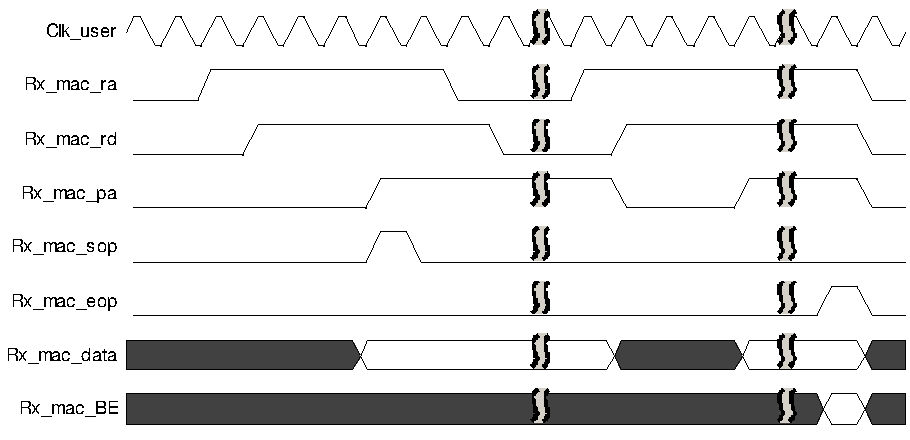
\includegraphics[width=0.9\textwidth]{Figures/oc_rx}
\caption[Timing diagram of the OpenCores ethernet\_tri\_mode IP core RX user interface]{Timing diagram of the OpenCores ethernet\_tri\_mode IP core RX user interface. Source:~\cite{OCMAC}}
\label{fig:oc_rx}
\end{figure}

As can be seen in the official documentation~\cite{OCMAC}, the user interface is documented only by two vague timing diagrams, one for transmission and one for reception, without any explanation of the signals involved. The fact that the user must resort to guesswork makes the core difficult to use. The RX part is included here without modification in \fref{fig:oc_rx}, the TX case is similar. The data bus \texttt{Rx\_mac\_data} is 32 bits wide. It is difficult to ascertain the meaning of the signals, but \texttt{Rx\_mac\_sop} is assumed to be the start of packet indicator while \texttt{Rx\_mac\_eop} looks like the end of packet indicator. They provide the actual length of the data only indirectly; the user needs to count how many bytes were transferred between assertion of the indicators if the size information is needed for further processing, which is very often the case. A look into the source code reveals that \texttt{Rx\_mac\_BE} serves as indicator for byte validity in the last 4-byte unit of packet data. As packets can have lengths that are not multiples of 4 bytes, the user has to put some effort into special handling of the last data unit. These considerations already show that the interface is more complex than it needs to be for general-purpose applications.

Another MAC implementation in the recent journal article ``Design and Implementation of an Ethernet MAC IP Core for Embedded Applications"~\cite{MAC_journal} has a similar aim of providing a flexible core for various applications. Because the full text could not be procured, only the abstract is considered here. It shows that the primary goal was to reduce FPGA resource usage and power consumption, which is deliberately not the case in the present thesis. The focus on ease of use and understanding here is a clear distinction from the work demonstrated in the article.

In summary, a sizable number of prior implementations exist but we have seen none that meet the goals of this thesis, especially being easy to use and understand and having the source code available free of charge.

\section{Hardware platform}\label{ch:hw_spartan}

\begin{figure}
\centering
\begin{tikzpicture}[
	every path/.style={line join=round,line cap=round},
	legend/.style={
		node font=\fontsize{13pt}{1em}\selectfont
	},
	fpga/.style={Tblue},
	ethcon/.style={Tred},
	phy/.style={Torange},
	marking/.style={line width=3.5pt},
	callout/.style={line width=1.5pt}
]
\node[anchor=south west,inner sep=0] (Image) at (0,0) {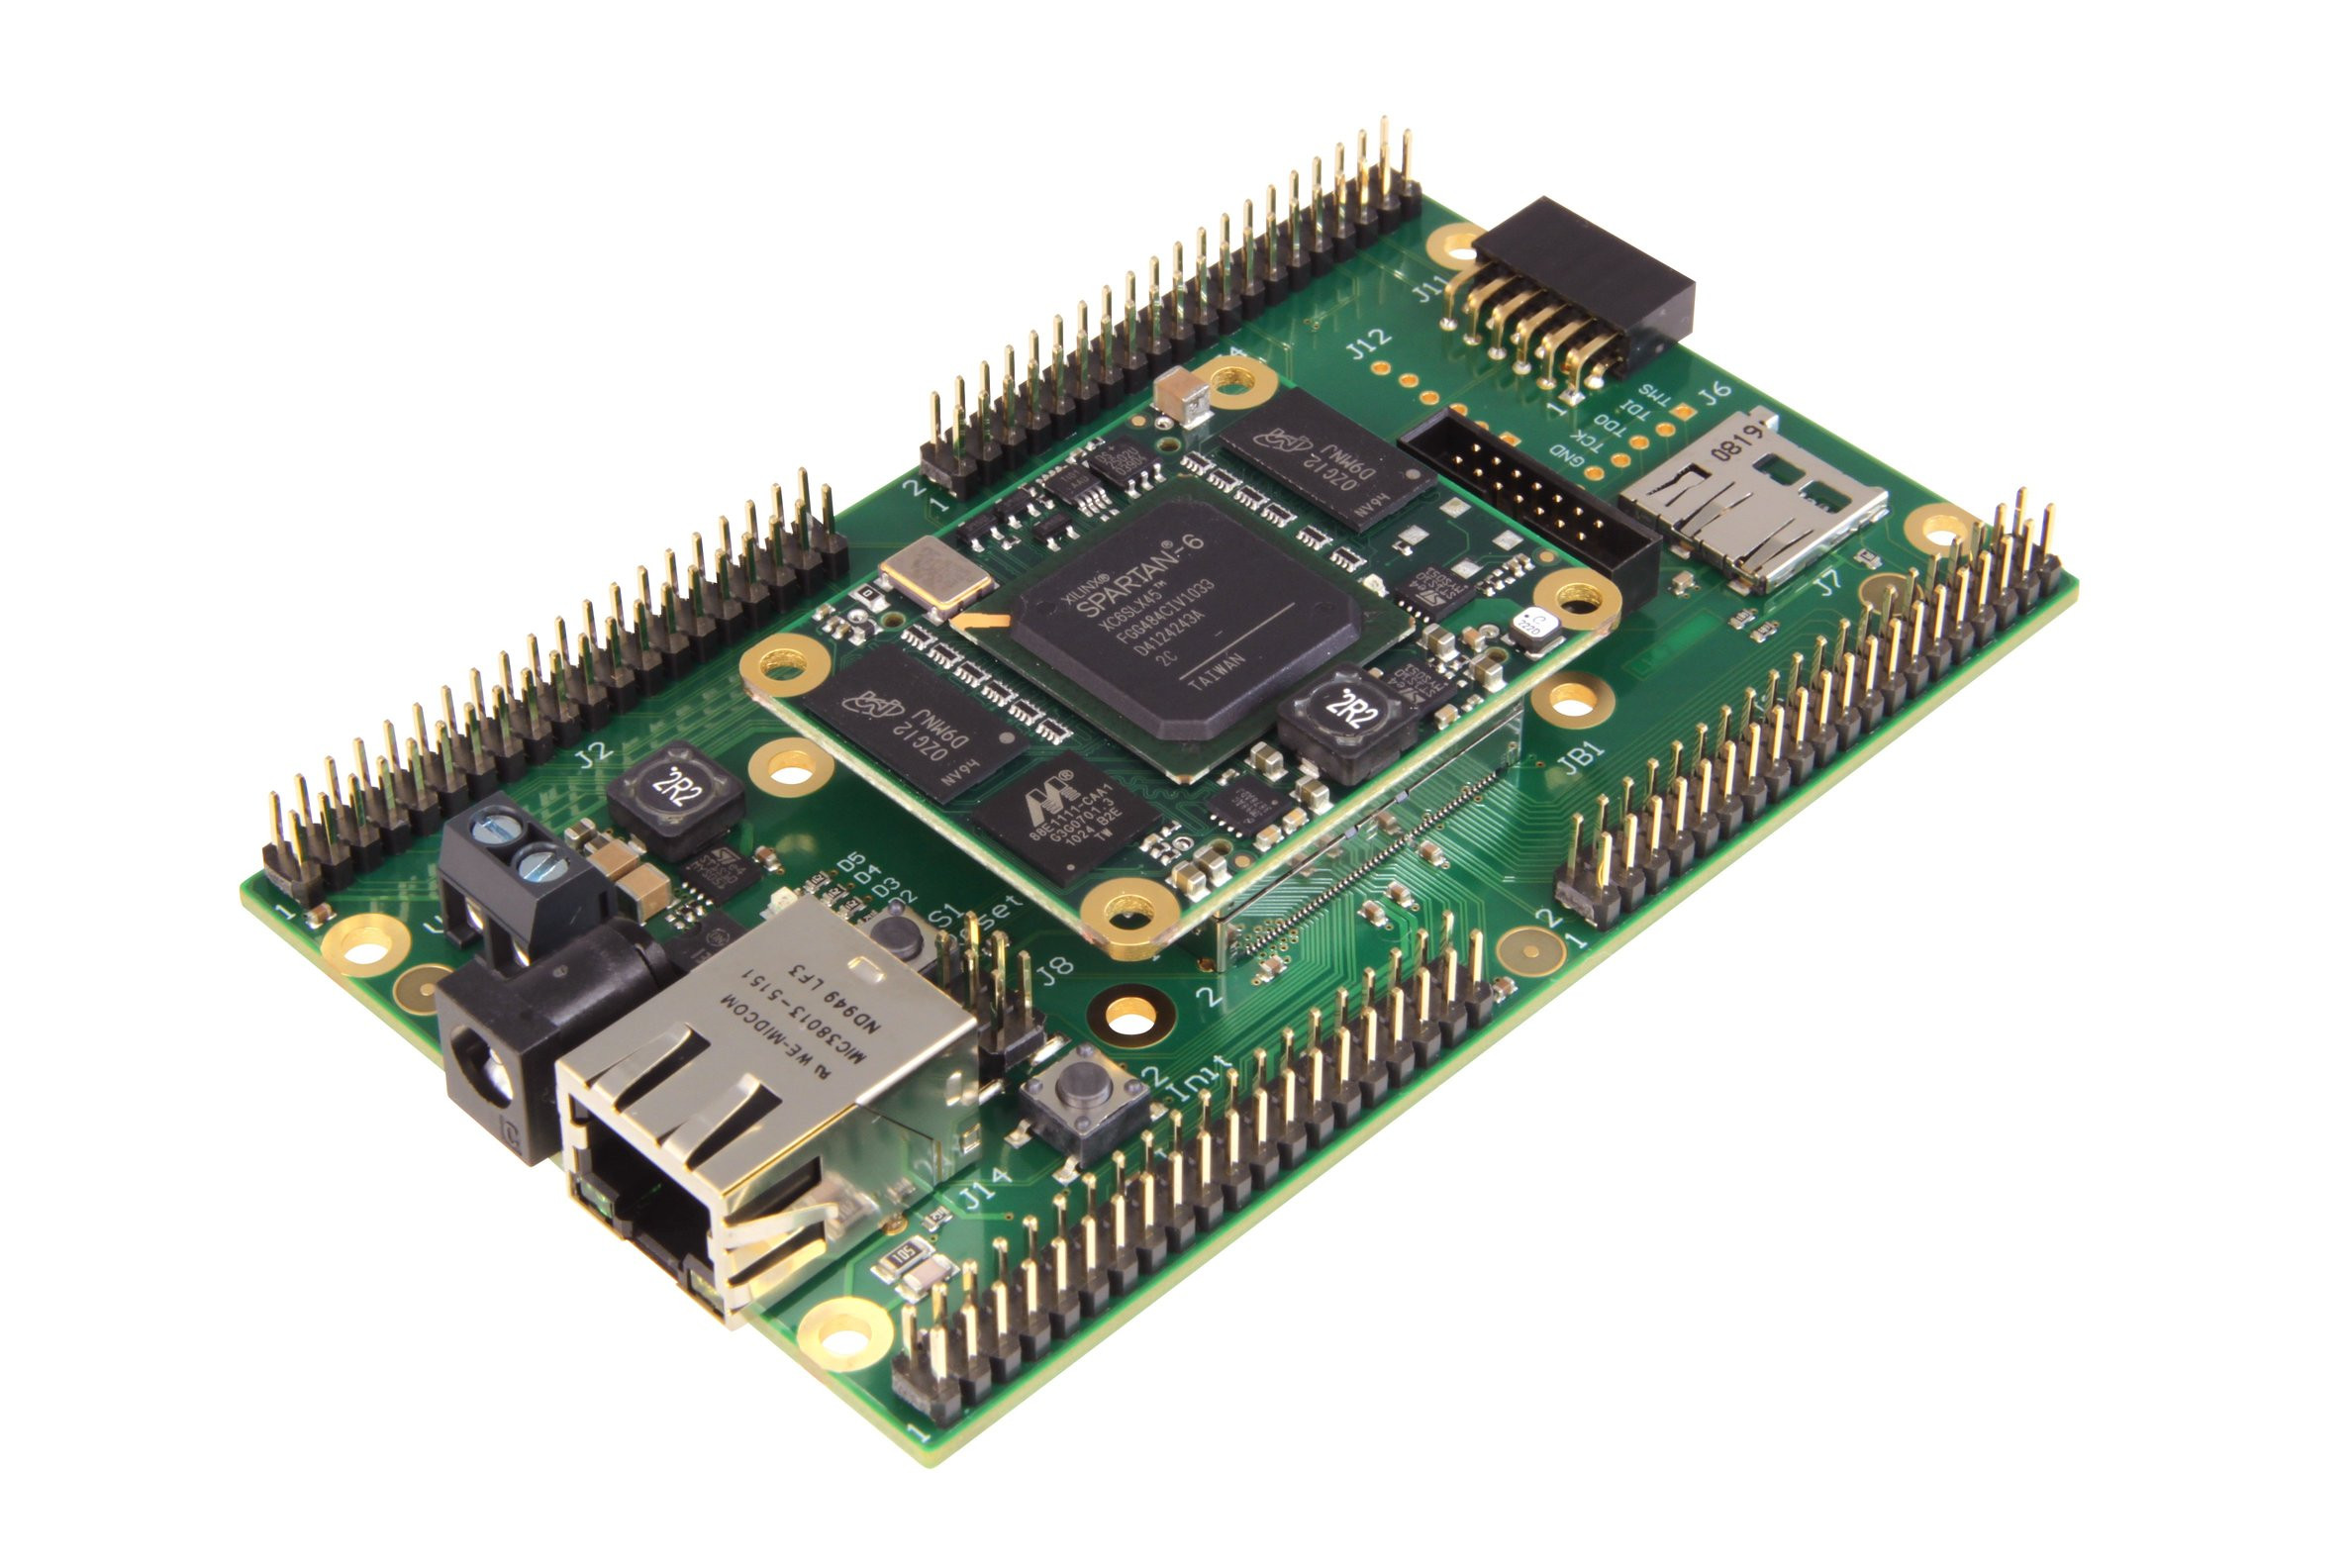
\includegraphics[width=0.8\textwidth]{Figures/TE603+TE600.angle.jpg}};
% Transform coordinate system to normal picture coordinates
\begin{scope}[x={(Image.south east)},y={(Image.north west)},yscale=-1,shift={($(Image.north) - (Image.south)$)}]
	%\draw[red,ultra thick] (0.26,0.12) rectangle (0.78,0.75);
	\node[legend,fpga] (FPGA) at (0.26,0.12) {Xilinx Spartan-6 family FPGA};
	\node[legend,ethcon,anchor=base] (EthCon) at (0.16,0.92) {Ethernet connector};
	\node[legend,phy,anchor=base] (PHY) at (0.72,0.92) {Marvell 88E1111 Ethernet PHY};
	
	\draw[marking,fpga] (0.505,0.508) -- (0.610,0.394) -- (0.505,0.293) -- (0.399,0.400) coordinate[midway] (FPGAEdge) -- cycle;
	\draw[callout,fpga] (FPGAEdge) -- (FPGA);
	\draw[marking,phy] (0.451,0.473) -- (0.498,0.521) -- (0.454,0.571) coordinate[midway] (PHYEdge) -- (0.407,0.520) -- cycle;
	\draw[callout,phy] (PHYEdge) -- (PHY);
	\draw[marking,ethcon] (0.345,0.564) -- (0.420,0.650) -- (0.421,0.742) -- (0.312,0.857) -- (0.236,0.768) coordinate[midway] (EthConEdge) -- (0.231,0.674) -- cycle;
	\draw[callout,ethcon] (EthConEdge) -- (EthCon);
\end{scope}
\end{tikzpicture}
\caption[Trenz Electronic TE0603 baseboard with a GigaBee XC6SLX series module mounted on top]{A Trenz Electronic TE0603 baseboard with a GigaBee XC6SLX series module mounted on top. Source:~\cite{GigaBeeImage} (component markings added).}
\label{fig:te0600}
\end{figure}

\sref{ch:fpgas} provided a general introduction to field-programmable gate arrays that is now expanded upon by introducing the specific device and environment used during development of the MAC sublayer implementation presented in this thesis. The primary target platform is a GigaBee XC6SLX series industrial-grade FPGA micromodule manufactured by Trenz Electronic GmbH~\cite{TE0600Page}. It includes a Xilinx Spartan-6 LX family FPGA at a system clock rate of 125~MHz and a 10/100/1000 tri-speed ethernet PHY chip Marvell Alaska 88E1111~\cite{TE0600} which supports a very wide range of interfaces: MII/GMII, RGMII, TBI, reduced pin count TBI (RTBI), and SGMII~\cite{MarvellPHY}. Which of those is used can be configured through the MII management interface. The smallest variant which is also the one used during development has a Xilinx XC6SLX45-2 FPGA and two 128 MiB dynamic random access memory (DRAM) ICs for data storage. As the micromodule cannot be used stand-alone, the optional baseboard TE0603 provides power supply circuitry and a standard Ethernet connector for testing purposes~\cite{TE0603}. It can be replaced by a custom printed circuit board in actual applications. \fref{fig:te0600} shows the two boards mated together.

The XC6SLX45 offers a total amount of 43,661 logic cells, 2,088~kB of block RAM storage, 8 digital clock managers (DCMs), and 4 phase locked loops (PLLs)~\cite{S6Family}. All Spartan-6 family FPGAs have 16 global clock buffers called BUFGMUX that must be used to get clock signals onto the clocking interconnect, each of which can switch between two input clocks by way of a third select input. The switch can be performed free of glitches provided both clocks are continuously running~\cite{S6Clocking}.

Furthermore, there are flip-flop elements located directly besides every device pin in their designated input/output blocks (IOBs) to provide outputs with low skew called OLOGIC2 and capture inputs directly at their source called ILOGIC2~\cite{S6SelectIO}. When combined with the possibility to also capture a clock right at the pin in a BUFIO2 element and use it to clock the FFs of neighboring data pins, input from high-speed data buses that supply their own clock signal can be easily implemented, eliminating delay and skew issues when the clock is first routed to a global buffer and then to a FF located arbitrarily in the device. The configurable delay element IODELAY2 again built into every IOB can be used to delay the clock, the data signal, or both in order to place the rising edge of the clock right in the middle of the valid data window. All I/O registers additionally provide double data rate ability. Buffers supporting a wide range of digital I/O standards are available. They drive either the general (input buffer IBUF, output buffer OBUF) or the clocking interconnect (input buffer IBUFG). There is no dedicated clock output buffer.

Up to this point, only preexisting technologies and products were introduced. Subsequently, this information is put to good use by moving on to the design and implementation of the FPGA-based Ethernet MAC sublayer.

\chapter{Design}\label{ch:design}

The first step in developing the Ethernet MAC was to partition the task into smaller components (VHDL entities) with distinct responsibilities and define their interconnection. Special attention is drawn to a few key points that we will discuss first before we take a look at the resulting design in \sref{ch:overview}. A more thorough look at each component follows in \sref{ch:components}.

\section{Design trade-offs}

The interface offered to the user is of primary concern: to reach the goals of this thesis, it has to be fast enough to allow for symmetrical 1~Gb/s data transfer but also be easy to use, i.e.\ use simple signals and a common pattern that hardware developers are inherently familiar with. Furthermore, the users should be able to freely choose the clock they want to use for communicating with the MAC to avoid implementing clock domain crossing - the MAC should do that for them. A standard on-chip system bus like the Advanced eXtensible Interface (AXI) by ARM Limited~\cite{AXI} or Wishbone by OpenCores~\cite{Wishbone} is unfeasible because even though the concept is certainly well-known, it is over-sized for simple applications both in terms of signal count and complexity. Already less complex but similar in the overall idea is a block of RAM which acts as a buffer. To transmit a packet, the user could write it into the memory, but then the following questions have to be considered: how does the transmission logic know where the next packet lies in the buffer? How does it know that a packet is ready to send? How does the user know which packets in the buffer were sent and where he or she can write the next bulk of data? These are questions that can be answered, but in the course of doing so the naively suggested RAM interface will inevitably become more complex. If we think back to \sref{ch:fifo} though, we remember the FIFO interface and its characteristic of being very simple. It is also well-known, allows for high-speed data transfer and, when backed by a standard implementation, offers easy clock domain crossing, making it ideal for the MAC sublayer presented in this thesis.

When describing an interface, not only the connections, but also the width and format of the data that is passed over them must be clear. To be able to construct a valid MAC frame, at least the destination address, source address, length/type, and client data is needed as we have seen in \sref{ch:eth_frames}. The preamble and start frame delimiter can be skipped as they do not carry any information anyway. Theoretically speaking, these fields can be encoded in any fashion and order. But for both the user and the implementation of the media access control sublayer, keeping it plain and sticking to the format already defined in the Ethernet standard is the easiest option. There is also nothing to be gained by being fancy about the frame data representation. By sticking to the standard, the MAC can pass through most of the frame without any modification.

There is one complication concerning the frame trailer though: on the one hand, the user should not have to include the padding and frame check sequence on transmission. This problem can be solved when the data is defined to end right before padding and the MAC takes care of adding it. On reception on the other hand, the original length of the frame is not necessarily part of the header and thus unknown, so the padding cannot be removed in the general case. The FCS is a fixed-length field at the end of the packet and thus can always be stripped. Doing so makes the interface as symmetrical as possible. The user then has no possibility of verifying the integrity of a received packet, but that is also not necessary when the MAC takes proper care that erroneous packets are internally consumed and never reach the FIFO interface.

We have yet to examine the question of how many bits to transfer in one clock cycle, but as Ethernet counts data in multiples of bytes, making the interface 8 bit wide is the natural choice. A wider data bus allows for lower interface clock rates at identical data rates, but necessitates adaption logic to guarantee that byte units can be received and transmitted. In a general-purpose MAC, it is impossible to know the exact requirements of the user and what width would benefit his or her application, so the design has to cover all possibilities with the least common denominator of 1 byte. Width conversion logic can be easily added on top of the MAC FIFO interface by the user if there is a need for it.

A problem that still lingers in the FIFO architecture is that if only the data of packets is passed on, there is no way to know where they start and end. This is fixed by placing two bytes that indicate the size of the next packet in the buffer before each data part. Ethernet frames can be up to 1514 bytes long (excluding the frame check sequence), so one byte (maximum value 255) would not be enough for storing their size; the next possibility is using two bytes (maximum value 65535). As $\lceil \log_2 1514 \rceil = 11$ bits are strictly needed for storing the maximally possible frame size, 5 of the 16 bits will inevitably remain unused but the wasted space is so small that it is of no concern. It accounts for between 0.04 and 1.02 percent of the total stored data, depending on the packet size.

Nevertheless, we can see that there are in fact two limitations with this simple approach:
\begin{enumerate}
\item Packets must be delayed in the FIFO until they have been completely received so their size is known and can be put in front of the data.
\item The user needs to know the sizes of packets prior to starting transmission. 
\end{enumerate}

Both are rarely relevant in practice: a packet can usually not be acted upon as it is still being received since it could contain errors that are only detected when the frame check sequence that follows the data payload is verified. It is very important to understand that only the latency is different but that the achievable RX data rate is identical both when delaying the packet and when handing it to the user immediately. As for the second restriction, most users will want to use protocols that include further header checksums like UDP/IP instead of raw Ethernet frames. The IP header for example includes a field for the length of the packet, so to calculate its checksum the packet size again has to be known beforehand no matter how the MAC sublayer is designed.

One of the other choices to be made is whether to have completely separate modules in the transmit and receive paths or to combine some or all of them. Either option is feasible as there is zero interaction between both directions. However, the functionality is very similar, symmetrical even, so the code will be easier to understand if it is kept in one place. Splitting it per direction serves little purpose besides artificially increasing the component count, complicating the design. The single exception where it is worthwhile to make a separation are the FIFOs. The user might want to replace only one direction with a custom implementation.
%We always have to keep in mind that the primary goal is to make the system as easy to understand as possible, but also as complex as necessary.

These were the key points that we need to take into account when studying the MAC design in the following section.

\section{Overview}\label{ch:overview}

\fref{fig:system} shows an overview of the MAC design. Every block corresponds to a VHDL entity with the indicated name. The arrows indicate conceptual flow of data and do \emph{not} imply VHDL port directions. We shortly discuss the diagram beginning at the interface to the user application on the left-hand side and continuing rightwards from there until reaching the connection to the physical layer on the right-hand side.

\begin{figure}
\centering
\begin{tikzpicture}[
	every node/.style={
		node font=\footnotesize
	},
	block/.style={
		draw=black,
		shade,
		shading=axis,
		top color=Tbluelight!50,
		bottom color=Tbluelight!80,
		rounded corners,
		align=center,
		minimum height=1.5cm,
		%minimum width=2cm,
		text width=1.5cm,
		node font=\ttfamily\footnotesize
	},
	devdep/.style={
		top color=Torangelight!30,bottom color=Torangelight!70
	},
	bus/.style={
		%double=white,
		double,
		line width=1pt,
		double distance=4pt
	},
	enclosure/.style={
		draw=black,
%		dashed,
		fill=Tlilaclight!20
	},
	busp/.tip={Implies[length=5mm,fill=white]},
	<->/.tip=Latex
]
	\pgfdeclarelayer{bg}
	\pgfsetlayers{bg,main}
	
	\def\nodesize{2cm}
	\def\nodeenclosuresep{0.4}
	\def\arrowsep{0.5}

	\node[block] (MII) {mii\_gmii};

	\node[block,left=of MII] (Framing) {framing};
	\node[block,right=of MII,devdep] (IO)  {mii\_gmii\_\\io};
	\node[block,below=of MII] (MIIMC) {miim\_\\control};
	\node[block,right=of MIIMC] (MIIM) {miim};
	
	\node[block,left=of Framing] (TXFIFO) {tx\_fifo};
	\node[block,below=of TXFIFO] (RXFIFO) {rx\_fifo};
	
	\path ($(TXFIFO.west)!.5!(RXFIFO.west)+(-1.5,0)$) node[rotate=90] {\large \bfseries User application};
	\path ($(IO.east)!.5!(MIIM.east)+(2,0)$) node[rotate=90] {\large \bfseries PHY};
	
	\draw[vecArrowStart] (TXFIFO.west) -- ++(-1cm,0) coordinate (TXFIFOArrowEnd);
	\draw[vecArrowEndTX] (TXFIFO.east) -- ++(0.5,0) |- ($(Framing.west)+(0,\arrowsep)$);
	\draw[vecArrowEndTX] ($(Framing.east)+(0,\arrowsep)$) -- ($(MII.west)+(0,\arrowsep)$);
	\draw[vecArrowEndTX] ($(MII.east)+(0,\arrowsep)$) -- ($(IO.west)+(0,\arrowsep)$);
	\draw[vecArrowEndTX] ($(IO.east)+(0,\arrowsep)$) -- ++(1.5cm,0);
	
	\draw[vecArrowEnd] (RXFIFO.west) -- ++(-1cm,0);
	\draw[vecArrowStartRX] (RXFIFO.east) -- ++(0.5cm,0) |- ($(Framing.west)+(0,-\arrowsep)$);
	\draw[vecArrowStartRX] ($(Framing.east)+(0,-\arrowsep)$) -- ($(MII.west)+(0,-\arrowsep)$);
	\draw[vecArrowStartRX] ($(MII.east)+(0,-\arrowsep)$) -- ($(IO.west)+(0,-\arrowsep)$);
	\draw[vecArrowStartRX] ($(IO.east)+(0,-\arrowsep)$) -- ++(1.5cm,0);
	
	\draw[->] (MIIMC) -- (MII) node [midway,above right] {\texttt{speed}} node [midway,linepoint] (SpeedMid) {};
	\draw[->] (SpeedMid) -- ++(-3.3,0) |- ($(RXFIFO.south west)+(-1,-0.7)$);
	\draw[->] (SpeedMid) -| (IO);
	\draw[->] (MIIMC) -- ++(-3,0) node [above,pos=0.5] {\texttt{link\_up}} |- ($(RXFIFO.south west)+(-1,-1)$);
	\draw[vecArrowStartMIIM,vecArrowEndMIIM] (MIIMC) -- (MIIM);
	\draw[vecArrowStartMIIM,vecArrowEndMIIM] (MIIM.east)  -- ++(1.5,0);
	
	\path ($(Framing.north west)+(-\nodeenclosuresep,2*\nodeenclosuresep)+(0,-0.1cm)$) coordinate (EthernetClockin);
	\draw [->] (EthernetClockin -| TXFIFOArrowEnd) -- (EthernetClockin) node[pos=1,above left] {125~MHz clock};
	\draw [->] (EthernetClockin -| TXFIFOArrowEnd) ++ (0,-0.5cm) -- ($(EthernetClockin) + (0,-0.5cm)$) node[pos=1,above left] {MIIM clock};
	
	\node [block,anchor=north west,node font=\footnotesize,minimum size=0.5cm,text width=] at ($(RXFIFO.south west) + (0,-4*\nodeenclosuresep)$) (IndepBlockLegendNode) {};
	\node [right=0.1cm of IndepBlockLegendNode] (IndepBlockLegend) {\footnotesize Device-independent VHDL entity};
	\node [right=0.4cm of IndepBlockLegend,block,devdep,minimum size=0.5cm,text width=] (DepBlockLegendNode) {};
	\node [right=0.1cm of DepBlockLegendNode] (DepBlockLegend) {\footnotesize Device-dependent VHDL entity};
	
	\draw [vecArrowEndTX] ($(IndepBlockLegendNode.south west) + (0,-\nodeenclosuresep)$) coordinate(TXCLKArrow) -- ++(1cm,0) node[right] (TXCLKText) {MII TX clock domain};
	\draw [vecArrowEndRX] ($(TXCLKText.east) + (0.3,0)$) coordinate(RXCLKArrow) -- ++(1cm,0) node[right] {MII RX clock domain};
	\draw [vecArrowEnd] ($(TXCLKArrow) + (0,-\nodeenclosuresep)$) -- ++(1cm,0) node[right] (UserCLKText) {User clock domains};
	\draw [vecArrowEndMIIM] ($(RXCLKArrow) + (0,-\nodeenclosuresep)$) -- ++(1cm,0) node[right] {MII management clock domain};
	
	\begin{pgfonlayer}{bg}
		\fill[enclosure] ($(TXFIFO.north west)+(-\nodeenclosuresep,4*\nodeenclosuresep)$) rectangle ($(MIIM.south east)+(2*\nodeenclosuresep,-3*\nodeenclosuresep)$);
		\fill[enclosure,fill=Tlilaclight!50,dashed] ($(Framing.north west)+(-\nodeenclosuresep,2*\nodeenclosuresep)$) rectangle ($(MIIM.south east)+(\nodeenclosuresep,-\nodeenclosuresep)$);
		\path ($(IO.north east)$) node [above left=0.2 and 0] {\texttt{ethernet}};
		\path ($(IO.north east)$) node [above left=0.2+2*\nodeenclosuresep and 0] {\texttt{ethernet\_with\_fifos}};		
	\end{pgfonlayer}

\end{tikzpicture}

\caption{Block diagram of the Ethernet MAC presented in this thesis}
\label{fig:system}
\end{figure}

To not require users to learn the details of the MAC implementation and buffer packets themselves, FIFOs with standard interfaces are provided for both the transmit and receive data paths as previously discussed. As can be seen in the diagram, the two directions are completely independent from each other throughout the whole design. The first entity that implements actual Media Access Control sublayer functionality is the \texttt{framing} component. Functionality-wise, it performs the core operations that are expected from an Ethernet MAC like generating and verifying checksums and packet encapsulation. The following \texttt{mii\_gmii} module acts as transparent converter between the generic streams of packet data and the actual signals expected by the media-independent interfaces as well as switching between MII and GMII as needed based on the current link speed. The speed is periodically read out of the MII management interface by \texttt{miim\_control} which also takes care of the initial configuration of the PHY after reset. Only the high-level functionality is allotted to this module while the actual MIIM interface transactions are performed by \texttt{miim}. Lastly, due to the narrow timing requirements of the MII/GMII connections, it is not possible to directly connect them to the FPGA package pins. The device-specific I/O configuration needed in between is provided by \texttt{mii\_gmii\_io}.

Besides the clock pins used by the MII, the MAC requires the user to supply a 125~MHz reference clock to use as transmission clock in GMII mode, a clock for the MII management interface, and two FIFO clocks, one for each direction. The latter three of these clocks can be identical to simplify the user design.
\clearpage
The \texttt{reset\_generator} entity (not shown in the figure) monitors the current link speed and issues a complete reset for the MII RX and TX clock domains when it changes. This guarantees a consistent system state after a potential transmission clock switch between MII and GMII. The reset indication is also provided to the user to ensure that no mismatched data is written to or read from the FIFOs. We will discuss the exact reasons why this procedure is necessary later when describing the IO implementation in \sref{ch:mii_io_tx}.

As a convenience for using the MAC core, all mentioned components beginning at \texttt{framing} are preconnected to each other in a structural entity called \texttt{ethernet} which is then combined again with the FIFOs to form \texttt{ethernet\_with\_fifos}. The latter is a ready-to-use entity offering the FIFOs' interfaces on the user side and direct MII connections on the PHY side. It can be instantiated in custom designs that want to use Ethernet without much effort. It generally does not provide any benefit to bypass the FIFOs and directly connect to the framing component except in sufficiently sophisticated applications.

To clarify how the components relate to the layered architecture defined in the Ethernet standard as introduced in \sref{ch:ethernet_overview}, \fref{fig:mac_layers} shows the Ethernet layers and selected entities of the MAC design presented in this thesis side-by-side. The higher layers on the right-hand side are only exemplary and can be exchanged for arbitrary user application layers. Although the purposes of the reconciliation sublayer (RS) and the original Ethernet MAC sublayer correspond to the \texttt{mii\_gmii} and \texttt{framing} entities respectively, the interfaces between them differ. The standard e.g. suggests that the RS and the MAC sublayer communicate data one bit at a time, which is impractical for actual implementation on an FPGA. Similar considerations apply to the interface the MAC offers to higher layers. The logical link control (LLC) sublayer is designated optional by the standard and must be implemented by the user if needed.

\begin{figure}
\centering
\begin{tikzpicture}[
	node distance=2pt,outer sep=0pt,
	layer/.style={
		draw=black,
		%fill=lightgray,
		shade,
		shading=axis,
		top color=Tgraylight3!40,
		bottom color=Tgraylight2,
		%rounded corners,
		align=center,
		text height=12pt,
		text width=2.5cm,
		text depth=5pt
	},
	ethlayer/.style={layer,
		text width=4.5cm
	},
	macimpl/.style={
		top color=Tlilaclight!40,
		bottom color=Tlilaclight!70
	},
	userimpl/.style={
		top color=Tbrownlight!50,
		bottom color=Tbrownlight!80
	},
	<->/.tip=Stealth
]
\node[ethlayer] (PHY) {PHY};
\node[ethlayer,above=1.3cm of PHY,text width=3cm,text height=8pt,text depth=3pt] (RS) {Reconciliation};
\draw[<->] (PHY) -- (RS) node[pos=0.5,anchor=east,align=right] {MII};
\node[ethlayer,above=of RS] (MAC) {MAC};
\node[ethlayer,above=of MAC] (LLC) {LLC or other MAC client};
%\node[ethlayer,bottom color=orange,below=0.7cm of PHY] (Med) {Medium};
%\draw[<->] (PHY) -- (Med) node[pos=0.5,anchor=east,align=right] {MDI};

\node[ethlayer,right=1.2cm of PHY] (T_PHY) {PHY};
\node[ethlayer,macimpl,above=1.3cm of T_PHY,text width=3cm,text height=8pt,text depth=3pt] (T_RS) {\texttt{mii\_gmii}};
\draw[<->] (T_PHY) -- (T_RS) node[pos=0.5,anchor=west,align=left] {MII \\ via \texttt{mii\_gmii\_io}};
\node[ethlayer,macimpl,above=of T_RS] (T_MAC) {\texttt{framing}};
\node[ethlayer,macimpl,above=of T_MAC] (T_LLC) {\texttt{tx\_fifo} and \texttt{rx\_fifo}};
\node[ethlayer,userimpl,above=1cm of T_LLC] (T_IP) {Network layer: IP};
\node[ethlayer,userimpl,above=of T_IP] (T_TCP) {Transport layer: TCP};
\node[ethlayer,userimpl,above=of T_TCP] (T_Wishbone) {Application: Wishbone};
%\node[ethlayer,bottom color=orange,below=0.7cm of T_PHY] (T_Med) {Medium};
%\draw[<->] (T_PHY) -- (T_Med) node[pos=0.5,anchor=east,align=right] {MDI};
\draw[<->] (T_IP) -- (T_LLC) node[pos=0.5,anchor=west,align=left] {User FIFO interface};

\node[above=of LLC,align=center] (Higher_Dots) {$\vdots$};
\node[align=center,anchor=south] at (Higher_Dots |- T_IP.south) (Higher) {Higher layers};
\node[above=0.3cm of T_Wishbone] (ethMAC) {\textbf{Present thesis}};
\node[anchor=base] at (Higher |- ethMAC.base) {\textbf{Ethernet layers}};

\draw (MAC.south east) -- (T_MAC.south west)
      (MAC.north east) -- (T_LLC.north west)
      (Higher.south east) -- (T_IP.south west)
      (Higher.north east) -- (T_Wishbone.north west);
      
\node[ethlayer,text width=,minimum size=0.4cm,text height=,text depth=,below=0.5cm of PHY.south west,anchor=north west,macimpl] (LegendNode_MacImpl) {};
\node[right=of LegendNode_MacImpl] (Legend_MacImpl) {\footnotesize Present MAC implementation};
\node[ethlayer,text width=,minimum size=0.4cm,text height=,text depth=,right=0.5cm of Legend_MacImpl,userimpl] (LegendNode_UserImpl) {};
\node[right=of LegendNode_UserImpl] (Legend_UserImpl) {\footnotesize Exemplary user application};
\draw [dotted] ($(PHY.south west)+(-0.3cm,-0.3cm)$) -- ($(T_PHY.south east)+(0.3cm,-0.3cm)$);
\end{tikzpicture}

\caption[Ethernet simplified layer architecture in relation to the MAC implementation presented in this thesis]{Ethernet simplified layer architecture in relation to the MAC implementation presented in this thesis. Ethernet side adopted from \cite[fig. 1-1]{Ethernet}.}
\label{fig:mac_layers}
\end{figure}

\section{Components}\label{ch:components}

Let us now take a closer look at each component and the input and output connections it exposes to its neighbors.

\subsection{FIFOs}\label{ch:design_fifos}

The only modules that the user will normally interact with directly are the transmit and the receive FIFO buffer. Consistent with our prior considerations, both have a standard interface as seen for instance with Chu \cite[280]{RTLHardwareDesign} with a data width of 8 bits and only one side facing the user. The TX FIFO can be written, the RX FIFO can be read by the user. They both have their own clock domain with the clock supplied by the user. The timing characteristics conform to the interface of first-word fall-through FIFOs generated by the Xilinx LogiCore IP FIFO generator~\cite{XilinxFIFO}.

To send a packet, first of all the FIFO must not be full. The application must put the 2-byte size of the packet into the buffer, most significant byte (MSB) first, then the least significant byte (LSB), after which precisely as many bytes of data as were indicated must follow. Keeping the structure identical to the Ethernet standard avoids unnecessary and costly rearrangements within the Ethernet packet when sending. As soon as the FIFO detects that the data for the next packet has been written completely, it starts passing the data on to the framing module.

Receiving a packet works analogously: \texttt{framing} writes an incoming packet to the buffer. After it has been received completely and without errors, the RX FIFO will indicate that it is not empty and the size and data can be read. As an added convenience, the FIFO will pretend to be empty for a few clock cycles after every packet even when technically more packets are available, so the user can sense the end of a transmission unit and does not need to count the data bytes while reading. During ongoing read-out of a packet, the FIFO never becomes empty. Although the interface is identical to that of a normal FIFO and the entity is called \texttt{rx\_fifo}, it cannot work like one internally. The packet size is known and written to the memory only after the last data byte has been received, but needs to be read out first, before the data, in clear violation of the first-in-first-out principle. Also, erroneous frames must be skipped without requiring the user to read them out.

\begin{figure}
\centering
{
\setlength{\fboxrule}{0pt}
\begin{subfigure}[b]{0.45\textwidth}
\fbox{\begin{tikzpicture}[commandnode/.append style={top color=Tredlight!10,bottom color=Tredlight!20},<->/.tip=Latex]
\node [decisionnode,text width=2.3cm] (ReadyDecision) {Frame ready?};
\node [commandnode,below=0.7cm of ReadyDecision] (WREN) {Assert \texttt{wr\_en}};
\node [commandnode,below=of WREN,text width=5.2cm] (SizeMSB) {Write MSB of size $n$ to \texttt{data}};
\node [commandnode,below=of SizeMSB,text width=5.2cm] (SizeLSB) {Write LSB of size $n$ to \texttt{data}};
\node [commandnode,below=of SizeLSB,text width=5.2cm] (Payload) {Write one byte of data to \texttt{data}};
\node [decisionnode,below=of Payload,text width=3cm] (Decision) {$n$ bytes written?};
\node [commandnode,below=0.7cm of Decision] (TXWREN_De) {Deassert \texttt{wr\_en}};
\draw[->] (WREN) -- (SizeMSB);
\draw[->] (SizeMSB) -- (SizeLSB);
\draw[->] (SizeLSB) -- (Payload);
\draw[->] (Payload) -- (Decision);
\begin{scope}[on background layer]
\draw[->] (ReadyDecision.center) -- (WREN) node[pos=1,above right] {Yes};
\draw[->] (ReadyDecision.center) -- (ReadyDecision.east) -- ++(0.4cm,0) node[pos=0,below right] {No} |- ($(ReadyDecision.north)+(0,0.3cm)$);
\draw[->] (Decision.center) -- (TXWREN_De) node[pos=1,above right] {Yes};
\draw[->] (Decision.center) -- (Decision.east) -- ++(1cm,0) node[pos=0,below right] {No} |- (Payload.east);
\end{scope}
\draw[->] (TXWREN_De) -- ++(0,-1cm) -- ++(3.5cm,0) |- ($(ReadyDecision.north)+(0,0.5cm)$) -- (ReadyDecision);
\end{tikzpicture}}
\caption{Transmission}
\label{fig:fifo_flow_tx}
\end{subfigure}
\begin{subfigure}[b]{0.45\textwidth}
% Placement of this figure is weird w/o fbox
\fbox{\begin{tikzpicture}[commandnode/.append style={top color=Tgreenlight!10,bottom color=Tgreenlight!20},<->/.tip=Latex]
\node [decisionnode,text width=2.3cm] (EmptyDecision) {\texttt{empty} = 0?};
\node [commandnode,below=0.7cm of EmptyDecision] (RDEN) {Assert \texttt{rd\_en}};
\node [commandnode,below=of RDEN,text width=5.5cm] (SizeMSB) {Read MSB of size $n$ from \texttt{data}};
\node [commandnode,below=of SizeMSB,text width=5.5cm] (SizeLSB) {Read LSB of size $n$ from \texttt{data}};
\node [commandnode,below=of SizeLSB,text width=5.5cm] (Payload) {Read one byte of data from \texttt{data}};
\node [decisionnode,below=of Payload,text width=3cm] (Decision) {\texttt{empty} = 1?};
\node [commandnode,below=0.7cm of Decision] (RXRDEN_De) {Deassert \texttt{rd\_en}};
\draw[->] (RDEN) -- (SizeMSB);
\draw[->] (SizeMSB) -- (SizeLSB);
\draw[->] (SizeLSB) -- (Payload);
\draw[->] (Payload) -- (Decision);
\begin{scope}[on background layer]
\draw[->] (EmptyDecision.center) -- (RDEN) node[pos=1,above right] {Yes};
\draw[->] (EmptyDecision.center) -- (EmptyDecision.east) -- ++(0.4cm,0) node[pos=0,below right] {No} |- ($(EmptyDecision.north)+(0,0.3cm)$);
\draw[->] (Decision.center) -- (RXRDEN_De) node[pos=1,above right] {Yes};
\draw[->] (Decision.center) -- (Decision.east) -- ++(1cm,0) node[pos=0,below right] {No} |- (Payload.east);
\end{scope}
\draw[->] (RXRDEN_De) -- ++(0,-1cm) -- ++(3.7cm,0) |- ($(EmptyDecision.north)+(0,0.5cm)$) -- (EmptyDecision);
\end{tikzpicture}
}
\caption{Reception}
\label{fig:fifo_flow_rx}
\end{subfigure}
}
\caption{Flowcharts for packet transmission and reception on the MAC's FIFO user interface}
\label{fig:fifo_flow}
\end{figure}

\fref{fig:fifo_flow} shows basic flowcharts for both transmission and reception of packets using the FIFO. The signal name \texttt{wr\_en} means ``write enable" while \texttt{rd\_en} stands for ``read enable". In the actual entities, the port names are additionally prefixed by the direction (\texttt{tx\_} or \texttt{rx\_}). Although it is not shown for the TX case (\fref{fig:fifo_flow_tx}) because it would considerably clutter the diagram, each write step can only occur when \texttt{tx\_full\_o} is not asserted. If it is, the user has to deassert \texttt{tx\_wr\_en\_i} and delay the byte until the FIFO has space available again, or the write will be lost.

\subsection{Framing}\label{ch:framing}

As the core part implementing actual MAC sublayer functionality, the \texttt{framing} component has the following responsibilities:

\begin{itemize}
\item \textbf{Encapsulation} of packets on transmission:
\begin{itemize}
\item Insertion of the preamble and start frame delimiter before transmitting the data
\item Insertion of padding as required
\item Calculation and insertion of the frame check sequence
\item Enforcement of the interpacket gap
\end{itemize}
\item \textbf{Verification and decapsulation} of packets on reception:
\begin{itemize}
\item Verification of the frame start which should be any number of preamble bytes followed by the start frame delimiter
\item Verification of the frame check sequence
\item Verification of the packet length which should be within the limits required by the Ethernet standard
\end{itemize}
\end{itemize}

All tasks are fulfilled by forwarding the data stream from the FIFO to \texttt{mii\_gmii} and vice-versa, carefully inserting and removing data bytes as necessary. The interface offered to the FIFOs is almost identical to the one towards the \texttt{mii\_gmii} module. \tref{table:framing_signals} lists all ports of the module. Transfer of a single byte of data can take a different amount of clock cycles depending on the underlying MII variant in use: only 4 bits can be transferred at a time with the Fast Ethernet MII for example, so it will take two cycles to completely send 8 bits. Since \texttt{mii\_gmii} does not buffer data, a new byte can only be placed on the line after the current one was processed. The next data unit should be placed on \texttt{tx\_data} in each clock cycle that has \texttt{tx\_byte\_sent} high when transmitting data, and read from \texttt{rx\_data} in each clock cycle that has \texttt{rx\_byte\_received} high when receiving data. The \texttt{tx\_byte\_sent} and \texttt{rx\_byte\_received} signals effectively act as a data strobe signal. Exemplary timing diagrams for packet transactions are found in \aref{ch:framing_timing}.

\begin{table}
\caption[Ports of the framing entity]{Ports of the \texttt{framing} entity}
\centering
\begin{tabu} to\linewidth {>{\ttfamily}XX[2]}
\rowfont[c]{\normalfont\bfseries} Port name & Function \\ \hline
tx\_reset\_i & Active-high asynchronous reset of all TX functions \\
tx\_clock\_i & Clock for all transmit signals \\
tx\_enable\_i & Active-high transmit enable \\
tx\_data\_i<7:0> & Data to transmit \\
tx\_byte\_sent\_o & Put next byte on \texttt{tx\_data} when asserted \\
tx\_busy\_o & Start new packet only when deasserted \\ \hline
rx\_reset\_i & Active-high asynchronous reset of all RX functions \\
rx\_clock\_i & Clock for all receive signals \\
rx\_frame\_o & Asserted as long as one continuous frame is being received \\
rx\_data\_o<7:0> & Data received \\
rx\_byte\_received\_o & Asserted when \texttt{rx\_data} is valid \\
rx\_error\_o & Active-high receive error indication \\ \hline
mii\_tx\_enable\_o & Function equivalent to \texttt{tx\_enable\_i} \\
mii\_tx\_data\_o<7:0> & Function equivalent to \texttt{tx\_data\_i} \\
mii\_tx\_byte\_sent\_i & Function equivalent to \texttt{tx\_byte\_sent\_o} \\
mii\_tx\_gap\_o & Transmit IPG when asserted \\
mii\_rx\_frame\_i & Function equivalent to \texttt{rx\_frame\_o} \\
mii\_rx\_data\_i<7:0> & Function equivalent to \texttt{rx\_data\_o} \\
mii\_rx\_byte\_received\_i & Function equivalent to \texttt{rx\_byte\_received\_o}\\
mii\_rx\_error\_i & Function equivalent to \texttt{rx\_error\_o} \\
\end{tabu}
\label{table:framing_signals}
\end{table}

All differences between the two sides of \texttt{framing} are related to the interpacket gap (IPG) in frame transmission: \texttt{tx\_busy} exists only towards the FIFO and \texttt{tx\_gap} only towards \texttt{mii\_gmii}. The busy indication is needed for signaling the FIFO to delay sending the next packet during the IPG while \texttt{tx\_gap} actively requests continued operation of \texttt{tx\_byte\_sent} without actually transmitting data on the media-independent interface.

Verification of incoming packets has two distinct ways in which errors are handled: should the frame beginning be invalid already, the remainder of the frame is silently skipped as no data has left \texttt{framing} yet. If the FCS or length checks fail, a reception error is indicated by \texttt{rx\_error\_o}. In any case, the FCS is not stripped from the packet on reception since doing so would require delaying the data stream by the checksum length of 4~bytes. This would substantially increase the complexity of the receive state machine. Instead, the \texttt{rx\_fifo} entity is responsible for removing the FCS before it reaches the user.

\subsection{Media-independent interface}

As the name \texttt{mii\_gmii} indicates, we have reached the first entity where actual communication with the physical layer device takes place. Because it primarily serves as a thin signal adaption layer, there is not much to do here, especially when GMII is used. Then the data received from \texttt{framing} can be passed on to the MII IO entity by directly mapping the ports. For MII though each data byte must be split into two 4-bit units on transmission and combined on reception. The MII signals \texttt{CRS}, \texttt{COL}, and \texttt{TX\_ER} are omitted from the MII/GMII ports because they are only useful in half-duplex modes.

\subsection{Media-independent interface input/output}

The outputs and inputs of the \texttt{mii} entity on the MII side already conform to the functional characteristics of the Ethernet specification, but their timing has to be adapted. Getting this right is dependent on the concrete FPGA architecture and as a consequence put into a separate exchangeable entity named \texttt{mii\_gmii\_io}. The ports must then finally be connected to the pins of the device by the user where they will reach the PHY.

\subsection{Media-independent interface management}

\texttt{miim} implements the standard management interface of MII. In addition to the actual MIIM \texttt{MDC} and \texttt{MDIO} signals for connection to the PHY, an interface to read and write single registers one at a time is provided. It runs in a user-supplied separate MIIM clock domain together with \texttt{miim\_control}.

\subsection{Media-independent interface management control}

For both the IO block and the MII/GMII interface adapter it is critical to know which speed is used on the physical medium because the PHY will only meaningfully process MII signals in 10 or 100~Mb/s operation and GMII signals in 1000~Mb/s operation. \texttt{miim\_control} leverages the \texttt{miim} entity to poll the status and auto-negotiation management registers which show if and at what speed a link is currently established. The speed information is propagated both MAC-internally and to the user. Whether a link has been established at all is irrelevant to the operation of the MAC; the indication is only provided for the user application. MII operation is completely stateless, so it is impossible to bring the interface into an invalid state. As long as the physical layer device has not successfully connected to a link partner, it will ignore transmission requests and not put any received packets on the RX interface.

The MAC sublayer will not support half-duplex connections, yet the PHY still needs to know that it should never try to establish a link at any such mode, which can be done via MIIM. The MIIM control entity thus is also responsible for configuring the physical layer device for full-duplex-only operation after reset.

\vskip\parskip\vskip\parskip

In this chapter, we discussed the abstract design of the MAC sublayer implementation, what decisions were made for design trade-offs and why. We can now go one step further and consider the actual VHDL implementation on a Xilinx Spartan-6 family FPGA.

\chapter{Implementation}\label{ch:implementation}

The task of implementing the system design presented in \cref{ch:design} means devising working, synthesizable VHDL code for each entity of the MAC core as well as their interconnections. For the verification purposes of this thesis, it is sufficient if it runs on a GigaBee module, but as was stated in the initial goals, the code should be flexible enough to allow for easy porting to other devices and vendors. In fact, the majority of it should be generic VHDL that does not use components specific to certain FPGA families at all. Some design entities such as the MII/GMII input/output architecture and the user FIFOs warrant special attention as their implementation needs more thought beyond just adhering to the specification. We will see how they are realized next.

The previous design choices were independent of the hardware description language used, as will many of the considerations relevant for implementation be. Generally, the focus is drawn to the ideas and concepts inherent to the source code rather than the concrete lines of code here. For some details that concern the goal of easy maintainability and understandability of the actual code, though, it is necessary to briefly discuss a few aspects of VHDL. As a general measure to make the code easier to grasp, a consistent coding style was applied throughout the source code; specific rules are found in \aref{ch:coding_style}. 

\section{(Gigabit) media-independent interface input/output}\label{ch:mii_io}

The only entity introduced as device-dependent was \texttt{mii\_gmii\_io} which implements the input/output part of MII and GMII. We will now see why this is not possible with generic HDL code and how it was concretely realized, starting with the transmission of Ethernet frame data.

\subsection{Transmission}\label{ch:mii_io_tx}

As explained in \sref{ch:eth_mii}, MII/GMII transmission clocking is complicated by the fact that two completely different clock sources must be used depending on the link speed. This and the need to meet the gigabit media-independent interface timing led to the structure seen in \fref{fig:mii_gmii_tx}. Note that the \texttt{mii\_gmii} TX logic block is only included for clarity and not part of \texttt{mii\_gmii\_io}.

\begin{figure}
\centering
\begin{tikzpicture}[circuit logic IEC,
%	/pgf/buffer gate IEC symbol=
miigmiitx/.style={
		miigmii,
		gLogic,
		gLogic ports=2:0:1:0,
		circuit symbol size=width 10 height 14,
}
]
	\pgfdeclarelayer{bg}
	\pgfsetlayers{bg,main}
	\def\pinlength{2\tikzcircuitssizeunit}
	\def\nodeenclosuresep{0.6cm}
	\def\pinsep{0.5cm}
	
	\node[bufgmux,rotate=180,minimum width=1cm] (CLKMUX) {};
	\node[below right=-0.1cm] at (CLKMUX.west) {\scriptsize\ttfamily S};
	\node[below left] at (CLKMUX.north) {\scriptsize\ttfamily O};
	\node[above left] at (CLKMUX.south east) {\scriptsize\ttfamily I0};
	\node[above left] at (CLKMUX.south west) {\scriptsize\ttfamily I1};

	% ODDR2
	\node[oddr,fill=white,below right=1cm and 2.5cm of CLKMUX,set gLogic west label={\scriptsize\ttfamily\ifcase#1 \or D0 \or D1 \or C0 \or C1 \or CE \fi},set gLogic east label={\scriptsize\ttfamily Q}] (ODDR_GTXCLK) {ODDR2};
	\node[inversion,anchor=east] at ($(ODDR_GTXCLK.wPin 3) + (\pinlength,0)$) {};
	\node[clockmarker,anchor=west] at ($(ODDR_GTXCLK.wPin 3) + (\pinlength,0)$) {};
	\node[clockmarker,anchor=west] at ($(ODDR_GTXCLK.wPin 4) + (\pinlength,0)$) {};
	
	\node[obuf,right=of ODDR_GTXCLK] (OBUF_GTXCLK) {};
	\draw (ODDR_GTXCLK.ePin 1) -- (OBUF_GTXCLK.input);
	
	\node[pin,miitx,signal to=east,right=\pinsep of OBUF_GTXCLK] (PIN_GTXCLK) {GTX\_CLK};
	\draw (OBUF_GTXCLK.output) -- (PIN_GTXCLK);
	
	% FDRE
	\foreach \txdnum/\preceding in {0/ODDR_GTXCLK,1/FDRE_TXD0} {
		\node[fdre,below=2cm of \preceding,set gLogic west label={\scriptsize\ttfamily\ifcase##1 \or D \or C \fi},set gLogic east label={\scriptsize\ttfamily Q}] (FDRE_TXD\txdnum) {FDRE};
		\node[clockmarker,anchor=west] at($(FDRE_TXD\txdnum.wPin 2) + (\pinlength,0)$) {};
		
		\node[obuf,right=of FDRE_TXD\txdnum] (OBUF_TXD\txdnum) {};
		\draw (FDRE_TXD\txdnum.ePin 1) -- (OBUF_TXD\txdnum.input);
		\node[pin,miitx,signal to=east, right=\pinsep of OBUF_TXD\txdnum] (PIN_TXD\txdnum) {TXD\txdnum};
		\draw (OBUF_TXD\txdnum.output) -- (PIN_TXD\txdnum);
		
		\begin{pgfonlayer}{bg}
			\fill[enclosure] ($(FDRE_TXD\txdnum.north west)+(-\nodeenclosuresep,\nodeenclosuresep)$) rectangle ($	(PIN_GTXCLK.south east |- FDRE_TXD\txdnum.south east)+(\nodeenclosuresep,-\nodeenclosuresep)$);
			\node[above left=\nodeenclosuresep and \nodeenclosuresep of FDRE_TXD\txdnum.north west,anchor=south west] {\texttt{TXD\txdnum} input/output block};
		\end{pgfonlayer}
	}
	
	% BUFGMUX to ODDR2 and FDRE
	\draw (CLKMUX.north) |- (ODDR_GTXCLK.wPin 3);
	\draw (CLKMUX.north |- ODDR_GTXCLK.wPin 3) node [linepoint] {} |- (ODDR_GTXCLK.wPin 4);
	\draw (CLKMUX.north |- ODDR_GTXCLK.wPin 4) node [linepoint] {} |- (FDRE_TXD0.wPin 2);	
	\draw (CLKMUX.north |- FDRE_TXD0.wPin 2) node [linepoint] {} |- (FDRE_TXD1.wPin 2);
	
	% ODDR2 D0 and D1
	\draw [-{Straight Barb[length=8pt,width=8pt]}] (ODDR_GTXCLK.wPin 1) -- ++(-0.5cm,0) node[above] {$V_{CC}$};
	\draw (ODDR_GTXCLK.wPin 2) -- ++(-0.5cm,0) coordinate(ODDR_GTXCLK_D1);
	\draw (ODDR_GTXCLK_D1) ++(0,0.2cm) -- ++(0,-0.4cm);	
	
	% TX_CLK input to BUFGMUX
	\node[ibufg,above left=of CLKMUX] (IBUF_TXCLK) {};
	\node[pin,miitx,signal to=east,left=of IBUF_TXCLK] (PIN_TXCLK) {TX\_CLK};
	\draw (PIN_TXCLK) -- (IBUF_TXCLK.input);
	\draw (IBUF_TXCLK.output) -| (CLKMUX.south east);
		
	% CLOCK_125 input to BUFGMUX
	\node[pin,signal to=east,above=1.4cm of PIN_TXCLK.west,anchor=west] (PIN_CLK125) {clock\_125\_i};
	\draw (PIN_CLK125) -| (CLKMUX.south west);
	
	% speed input to BUFGMUX
	\node[pin,signal to=east,above=of PIN_CLK125.west,anchor=west] (PIN_SPEED) {speed\_select\_i<1>};
	\draw (PIN_SPEED.east) -- ++(0.8cm,0) coordinate(PIN_SPEED_LINE) |- (CLKMUX.west);
	% speed_select to ODDR2
	\draw (PIN_SPEED_LINE |- CLKMUX.west) node[linepoint] {} |- (ODDR_GTXCLK.wPin 5);
	
	% mii_gmii
	\node[miigmiitx,below left=-3cm and 4cm of ODDR_GTXCLK,align=center,
		set gLogic west function={0.2},
		set gLogic east function={ifthenelse(#1<2,0.8,0.65)},
		set gLogic west label={\scriptsize\texttt{clock\_tx\_i}},
		set gLogic east label={\scriptsize\texttt{mii\_txd\_o<\pgfmathprint{int(#1-1)}>}}
	] (MII_GMII) {\texttt{mii\_gmii}\\TX logic};
	\node[clockmarker,anchor=west] at($(MII_GMII.wPin 1) + (\pinlength,0)$) {};
	\draw (MII_GMII.ePin 1) -- ++(1.0cm,0) |- (FDRE_TXD0.wPin 1);
	\draw (MII_GMII.ePin 2) -- ++(0.7cm,0) |- (FDRE_TXD1.wPin 1);
	\draw (CLKMUX.north) ++ (0,-0.5cm) -- ++ (-6.0cm,0) node[linepoint,pos=0] {} |- (MII_GMII.wPin 1);
	\draw (MII_GMII.wPin 1) node[linepoint] {} |- ++(\pinlength,-3.5cm) node[pin,signal to=east,anchor=west] (PIN_CLKOUT) {clock\_tx\_o};
	
	% ...
	\node[below left=0.7cm and 0 of FDRE_TXD1,anchor=north west,align=left] {$\vdots$ \\ repeat for \texttt{TXD<2:7>} and \texttt{TX\_EN}};
	\node[below=0.2cm of MII_GMII.ePin 2] {$\vdots$};

	% enclosures
	\begin{pgfonlayer}{bg}
		\fill[enclosure] ($(ODDR_GTXCLK.north west)+(-\nodeenclosuresep,\nodeenclosuresep)$) rectangle ($(PIN_GTXCLK.south east |- ODDR_GTXCLK.south east)+(\nodeenclosuresep,-\nodeenclosuresep)$);
		\node[above left=\nodeenclosuresep and \nodeenclosuresep,anchor=south west] at ($(ODDR_GTXCLK.north west)$) {\texttt{GTX\_CLK} input/output block};
	\end{pgfonlayer}

%  \node[gLogic,
%    gLogic ports=8:0:6:0,
%    align=center,
%    set gLogic west function={ifthenelse(#1<4,#1,(#1+2))/9},
%    set gLogic east label={\scriptsize$Y_{\pgfmathprint{int(\eports-#1+1)}}$},
%    set gLogic west label={\scriptsize\ifnum#1<4\pgfmathprint{Alph(#1)}\else$E_{\pgfmathprint{int(#1-3)}}%$\fi}] (n) {R2D2-\\Decoder};
%  \draw (n.ePin 1) to[bend right] (n.ePin 8);
%  \draw (n.wPin 1) to [bend right] (n.wPin 3);
%
%  \node[gLogic, circuit symbol size=width 4 height 8] (m) at (4,0) {};
%  \draw (m.ePin 1) to [bend right] (m.ePin 2);
%  \draw (m.wPin 1) to [bend right] (m.wPin 2);
%
%  \draw[line cap=rect] (n.ePin 2) --++ (right:.5cm) |- (m.sPin 1);
\end{tikzpicture}
\caption[Structure of the transmission part of mii\_gmii\_io on Spartan-6 family FPGAs]{Structure of the transmission part of \texttt{mii\_gmii\_io} on Spartan-6 family FPGAs}
\label{fig:mii_gmii_tx}
\end{figure}

The flip-flops in the Spartan-6 FPGAs do not have the ability to switch between different clock signals, but the global clock buffers (BUFGMUX) do. One of them is used for generating the \texttt{clock\_tx} signal necessary for the TX logic and output. The first input \texttt{I0} is the MII \texttt{TX\_CLK} pin buffered by an IBUFG clock input buffer that provides a relatively direct connection to the multiplexer. The second input \texttt{I1} needs to be a user-provided 125~MHz reference clock which is called \texttt{clock\_125}. Where this signal comes from is not important, it might for example also come directly from another input pin (although there are restrictions on which pins can be used in this case), or be generated by a digital clock manager from a system clock with differing frequency. What does matter is that it should not already be the output of another global clock buffer as cascading them results in the usage of general-purpose routing for the connection~\cite{S6Clocking}. Which of those two clocks is put on the output \texttt{O} is decided by the select input \texttt{S}. The most significant bit of the \texttt{speed\_select} signal generated by the MII management interface control component indicates whether the PHY currently operates at gigabit speed (logic high) or 10 or 100 megabit speed (logic low). This is exactly what is needed for the \texttt{S} input, no further conversion is necessary. The correct TX clock is then provided by the \texttt{mii\_gmii\_io} entity on the \texttt{clock\_tx\_o} port for the transmission logic throughout the MAC.

The Ethernet standard does not specify whether the MII \texttt{TX\_CLK} continues running in GMII mode when both interfaces are supported, thus we have to assume that it stops on transition to gigabit speed. This means that the BUFGMUX can not be operated in synchronous glitch-free mode. Switching asynchronously between clocks implicates that glitches can occur on the resulting clock signal e.g. when changing from a clock that has just fallen to one that is just about to rise, possibly violating timing requirements in every circuit that uses the signal. The consequences are metastability and an inconsistent system state. To get the MAC back into a defined state, the \texttt{reset\_generator} component initiates a complete reset of the core whenever it detects a speed change.

When the 125~MHz clock is used in GMII mode, it is necessary to output the TX clock for the PHY on the \texttt{GTX\_CLK} pin. Connecting the signal directly to an output buffer makes for a sub-optimal solution due to routing restrictions in the Spartan-6 family FPGAs. If the design is routable at all, the output may exhibit high delay and skew issues. The technique recommended by Xilinx in its ISE design suite is to use a double data rate output register ODDR2, connect the desired clock to the first clock input \texttt{C0}, and its inverse to the second clock input \texttt{C1}. We will discuss later why the exact opposite was done here. Each time a rising edge is detected on \texttt{C0}, the value of the input \texttt{D0} is put on the output \texttt{Q}. Similarly, a rising edge on \texttt{C1} (which is equal to a falling edge on \texttt{C0} since both are the inverse of each other here) puts \texttt{D1} through. Fixing \texttt{D0} to a logic one and \texttt{D1} to a logic zero then leads to a clock signal on \texttt{Q} that is identical to the input \texttt{C0} save for the delay induced by the register and the output buffer. To avoid outputting an unused high-frequency signal in MII mode when \texttt{GTX\_CLK} is not used, the clock enable input \texttt{CE} of the ODDR2 instance is connected to the speed indicator. When it is at logic low for 10/100~Mb/s link speed, the output will stop toggling.

For the TX signal lines \texttt{TXD<0:7>} and \texttt{TX\_EN}, we need to take special care to meet the GMII timing requirements of 2.5~ns setup time and 0.5~ns hold time with respect to the rising edge of \texttt{GTX\_CLK}. Connecting the flip-flops that generate the final output values inside the FPGA logic slices directly to the output buffers results in high routing skew between the bus signals and an unclear timing relation to the clock output pin. Utilizing the OLOGIC2 output flip-flops integrated into the input/output blocks, however, eliminates any larger skew as the routing delay between the flip-flop and the buffer located in the same IOB is close to identical for all signals. The relation to the \texttt{GTX\_CLK} output is also clear: although the HDL primitive for a D-type flip-flop with synchronous reset FDRE is different from the ODDR2 primitive used for the clock signal, both end up in OLOGIC2 blocks here, using the same hardware. The delay from a rising edge on the TX clock to the register input value appearing on the device pin for any TX signal including the output clock is thus almost equal. With this structure, the data pins will change when \texttt{GTX\_CLK} rises and are almost guaranteed to violate the hold time requirement. Actually, the opposite should be done: if the outputs change on the falling edge of the clock, both the setup and hold time is met and there is still a 1.5~ns setup margin for bus skew. This is easily achieved by swapping the \texttt{C0} and \texttt{C1} input pins of the ODDR2 instance used for \texttt{GTX\_CLK}, thereby inverting the clock output.

The aforementioned considerations were only valid for gigabit speed, but the resulting solution can be used without modifications for plain MII, too. It mandates a setup time of 15~ns and a hold time of 0~ns. Put differently, with a 25~MHz interface clock at 100~Mb/s link speed, 25~ns are available for the propagation of a rising edge on \texttt{TX\_CLK} through the input and global clock multiplexer to the clock input pin of the output flip-flops and from there for the propagation of the FF input signal to the device pin. All component and routing delays are small enough to meet this requirement without special intervention.

As different aspects need to be discussed for the reception case, it can not be implemented analogously and warrants a closer inspection.

\subsection{Reception}

To begin with a simplification compared to the transmission structure, the same interface clock is used for both MII and GMII. In contrast, other points get more complicated: for GMII output, 5~ns of the 8~ns clock period are available for transitioning the data signals. The opposite is true for the input case: the pins need to be sampled within a short window of 2~ns, not even 3~ns as one would assume because the Ethernet standards mandates differing timing requirements for the sender and the receiver to account for propagation delay mismatch between the clock and signal lines~\cite{Ethernet}. A prerequisite for matching the timing at all is that the Spartan-6 family IOB input flip-flops allow for combined setup and hold times of shorter than 2~ns, which they do. Depending on the speed grade of the device, the duration for which the signal has to stay stable is between 0.9~ns and 0.3~ns~\cite{S6DS}. The key problem is making sure that the rising edge of the \texttt{RX\_CLK} clock reliably arrives at the capture flip-flops when the centers of the data validity window of the signal lines and the flip-flop input window requirement line up. 

Skew is usually the engineer's enemy, but here we can use it to our advantage: controlled insertion or removal of skew between the clock and signal paths is required. Possibilities to achieve this include (in order of complexity):

\begin{itemize}
\item Trying to set timing constraints on the FPGA input pins in the design and letting the hardware synthesizer figure out how to make ends meet. As design tools are generally not advanced enough to devise complicated IO clocking schemes and using only routing delays comes with a number of limitations, this will most likely fail.
\item Using a digital clock manager or PLL to induce a defined phase shift on the clock. 10~Mb/s operation is not supported in this case as the minimum input frequencies for both the DCM (5~MHz) and the PLL (19~MHz)~\cite{S6DS} are well above the 2.5~MHz required.

A switch between 25~MHz and 125~MHz interface clock rate when the PHY changes speeds will cause the clock output to become incoherent with the interface clock until the DCM/PLL regains its locking state, but only for a short time of 5~ms at maximum. A loss of link also allows the device to increase the time between two rising edges from 8~ns up to 16~ns according to the IEEE standard~\cite{Ethernet}, leading to the same situation. Both conditions should only occur on initial connection of the link or when errors emerge at the physical layer. Under those circumstances however, frames must be expected to get lost until the link is stable, so the small recovery time of the clock manager is of no concern.

The clock may also be stretched or shortened by the PHY when it transitions between its reference clock and the clock recovered from the medium. Although the standard does not explicitly state it for the MII and GMII interfaces, with the most commonly used copper Ethernet variants 100BASE-TX and 1000BASE-T this should only happen in half-duplex operation. The stream and therefore clocking on the physical medium in full-duplex mode is continuous as long as power-saving capabilities are not specifically enabled.
\item Using the dedicated IO clocking buffer BUFIO2 that provides minimum delay routing at low skew for the clock and inserting an IODELAY2 element into each data signal path to compensate for its propagation delay. The delay time is configurable, so in theory, the value could be exactly matched to the signal setup time and the time needed for the clock to propagate through the BUFIO2 to the clock pin. In practice though, ``the Spartan-6 FPGA delay line is not compensated for either temperature or voltage"~\cite{S6SelectIO}, which means that the exact delay time varies greatly depending on the operating conditions.
\item Combining a DCM or PLL for 1000~Mb/s GMII operation with a simple buffer of \texttt{RX\_CLK} for 10/100~Mb/s MII operation and switching the clock source for the capture flip-flop as needed with a BUFGMUX clock multiplexer. The DCM/PLL with its configurable phase shift guarantees that timing is reliably met for Gigabit Ethernet, but is bypassed for interface clock speeds that it does not support and, in fact, is not needed for. MII has much more lenient timing requirements of 10~ns setup and 10~ns hold time that can be met without any special arrangements. The issue with the clock manager losing its lock on the clock signal when the PHY decides to stretch or short a pulse stays.
\end{itemize}

None of the proposed solutions is completely satisfactory. The last one is the most reliable option, but at the same time, it is also the most complex and requires a DCM or PLL, of which only a small number are available in the XC6SLX45, and they might be needed by the application using the MAC core. Using BUFIO2 and delay lines is straightforward and only requires one of 32 IO clocking buffers. The IODELAY2 elements are always associated with exactly one device pin and can not be used for another purpose by the user anyway. We see the resulting RX structure of \texttt{mii\_gmii\_io} in \fref{fig:mii_gmii_rx}. The BUFIO2 element also provides a second output clock that can be put on the global clocking interconnect by a global clock buffer BUFG. All reception logic in the design uses this clock to capture the MII interface data from the IO flip-flops. Again, the \texttt{mii\_gmii} RX logic block is not part of \texttt{mii\_gmii\_io} and only included for clarity.

\begin{figure}
\centering
\begin{tikzpicture}[circuit logic IEC,
bufio/.style = {
		gLogic,
		gLogic ports=2:0:1:0,
		circuit symbol size=width 7 height 7,
		fill=white
},
iodelay/.style = {
	gLogic,
	gLogic ports=1:0:1:0,
	set gLogic west label={\scriptsize\ttfamily IDATAIN},
	set gLogic east label={\scriptsize\ttfamily DATAOUT},
	circuit symbol size=width 8 height 4,
	fill=white
},
miigmiirx/.style={
		miigmii,
		gLogic,
		gLogic ports=0:0:3:0,
		circuit symbol size=width 10 height 14
}
%	/pgf/buffer gate IEC symbol=
]
	\pgfdeclarelayer{bg}
	\pgfsetlayers{bg,main}
	\def\pinlength{2\tikzcircuitssizeunit}
	\def\nodeenclosuresep{0.5cm}
	\def\pinsep{0.5cm}
	
	% RX_CLK
	\node[pin,miirx,signal to=east] (PIN_RXCLK) {RX\_CLK};
	\node[ibufg,right=\pinsep of PIN_RXCLK] (IBUF_RXCLK) {};
	\draw (PIN_RXCLK) -- (IBUF_RXCLK);
	\node[bufio,right=of IBUF_RXCLK,
		set gLogic west label={\scriptsize\ttfamily I},
		set gLogic east label={\scriptsize\ttfamily \ifcase#1 \or IOCLK \or DIVCLK \fi}
	] (BUFIO) {BUFIO2};
	\draw (IBUF_RXCLK) -- (BUFIO.wPin 1);
	\node[bufg,right=of BUFIO.ePin 2] (BUFG) {};
	\draw (BUFIO.ePin 2) |- (BUFG.input);
	
	% FDRE
	\foreach \rxdnum/\preceding in {0/PIN_RXCLK.west |- BUFIO.south,1/PIN_RXD0.west |- FDRE_RXD0.south} {
		\node[pin,miirx,signal to=east,below=2.5cm of \preceding,anchor=west] (PIN_RXD\rxdnum) {RXD\rxdnum};
		\node[ibuf,right=\pinsep of PIN_RXD\rxdnum] (IBUF_RXD\rxdnum) {};
		\draw (PIN_RXD\rxdnum) -- (IBUF_RXD\rxdnum.input);
		\node[iodelay,right=of IBUF_RXD\rxdnum,anchor=wPin 1] (IDELAY_RXD\rxdnum) {IODELAY2};	
		\draw (IBUF_RXD\rxdnum.output) -- (IDELAY_RXD\rxdnum.wPin 1);
		\node[fdre,right=of IDELAY_RXD\rxdnum.ePin 1,anchor=wPin 1,set gLogic west label={\scriptsize\ttfamily\ifcase##1 \or D \or C \fi},set gLogic east label={\scriptsize\ttfamily Q}] (FDRE_RXD\rxdnum) {FDRE};
		\node[clockmarker,anchor=west] at($(FDRE_RXD\rxdnum.wPin 2) + (\pinlength,0)$) {};
		\draw(IDELAY_RXD\rxdnum.ePin 1) -- (FDRE_RXD\rxdnum.wPin 1);
		
		\begin{pgfonlayer}{bg}
			\fill[enclosure] ($(PIN_RXD\rxdnum.north west |- FDRE_RXD\rxdnum.north)+(-\nodeenclosuresep,\nodeenclosuresep)$) rectangle ($	(FDRE_RXD\rxdnum.south east)+(\nodeenclosuresep,-\nodeenclosuresep)$);
			\node[above left=\nodeenclosuresep and \nodeenclosuresep of PIN_RXD\rxdnum.north west |- FDRE_RXD\rxdnum.north,anchor=south west] {\texttt{RXD\rxdnum} input/output block};
		\end{pgfonlayer}
	}
	
	\draw (FDRE_RXD0.wPin 2) -- ++(-0.1cm,0) node[linepoint] (FDRE_RXD0_CLKSPLIT) {} |- (BUFIO.ePin 1);
	\draw (FDRE_RXD0_CLKSPLIT) |- (FDRE_RXD1.wPin 2);
	
%				
	% mii_gmii
	\node[miigmiirx,right=3cm of BUFG,anchor=wPin 1,align=center,
		set gLogic west function={#1/7},
		set gLogic west label={\scriptsize\ifcase#1 \or \texttt{clock\_rx} \else \texttt{mii\_rxd\_i<\pgfmathprint{int(#1-1)}>} \fi}
	] (MII_GMII) {\texttt{mii\_gmii}\\RX logic};
	\node[clockmarker,anchor=west] at($(MII_GMII.wPin 1) + (\pinlength,0)$) {};
	\node[pin,signal to=east,above=0.4cm of MII_GMII.north west,anchor=south west] (PIN_CLOCKRX) {\texttt{clock\_rx\_o}}; 
	\draw (MII_GMII.wPin 1) ++(-1cm,0) node[linepoint] {} |- (PIN_CLOCKRX.west);
	
	\draw (BUFG.output) -- (MII_GMII.wPin 1);
	\draw (FDRE_RXD0.ePin 1) -- ++(0.2cm,0) |- (MII_GMII.wPin 2);
	\draw (FDRE_RXD1.ePin 1) -- ++(0.5cm,0) |- (MII_GMII.wPin 3);
%	\draw (MII_GMII.ePin 1) -- ++(1.5cm,0) |- (FDRE_TXD0.wPin 1);
%	\draw (MII_GMII.ePin 2) -- ++(1.2cm,0) |- (FDRE_TXD1.wPin 1);
%	\draw (CLKMUX.north) ++ (0,-0.5cm) -- ++ (-6.3cm,0) node[linepoint,pos=0] {} |- (MII_GMII.wPin 1);
%	\draw (MII_GMII.wPin 1) node[linepoint] {} -- ++(0,-3cm) node[pin,rotate=-90,signal to=east,anchor=west] (PIN_CLKOUT) {clock\_tx\_o};
%	
	% ...
	\node[below=0.5cm of PIN_RXD1.west |- FDRE_RXD1.south,anchor=north west,align=left] {$\vdots$ \\ repeat for \texttt{RXD<2:7>}, \texttt{RX\_EN}, and \texttt{RX\_ER}};
	\node[below right=0.2cm and 0 of MII_GMII.wPin 3] {$\vdots$};
	
	% enclosures
	\begin{pgfonlayer}{bg}
			\fill[enclosure] ($(PIN_RXCLK.west |- BUFIO.north)+(-\nodeenclosuresep,\nodeenclosuresep)$) rectangle ($(IBUF_RXCLK.east |- BUFIO.south)+(\nodeenclosuresep,-\nodeenclosuresep)$);
			\node[above left=\nodeenclosuresep and \nodeenclosuresep of PIN_RXCLK.north west |- BUFIO.north,anchor=south west] {\texttt{RX\_CLK} input/output block};
	\end{pgfonlayer}
\end{tikzpicture}
\caption[Structure of the reception part of mii\_gmii\_io on Spartan-6 family FPGAs]{Structure of the reception part of \texttt{mii\_gmii\_io} on Spartan-6 family FPGAs}
\label{fig:mii_gmii_rx}
\end{figure}

Due to the way the IO clocking is routed inside the device, some constraints apply to the MII/GMII RX pin placement beyond the limitation that \texttt{RX\_CLK} must be put on a global clock input pin which is true for all possible solutions. All RX interface signal pin locations must additionally belong to the same BUFIO2 clocking region. The exact extent of those regions is described in detail in the clocking user guide~\cite{S6Clocking}, but it should generally not be a problem for the user to meet this requirement. The primary target platform of this thesis - the Trenz Electronic GigaBee module - allows for this option.

We still have to address the major downside of this implementation variant: setting a delay value that guarantees reliable operation under all conditions. The IODELAY2 element can be configured with the IDELAY\_VALUE parameter, an integer between 0 and 255, that determines how much delay is applied to the signal. How this number maps to the time domain is not stated in the SelectIO user guide~\cite{S6SelectIO}, so it must be found by trial and error. After implementing a design, the static timing report generated by the Xilinx ISE tool suite shows how long the delay applied actually is.

The total delay of the RX clock from the device pin until the final flip-flop input port is at least 1.7~ns under optimum conditions and at most 3~ns under worst-case conditions on the reference board according to the timing report. The input FF in the Spartan-6 FPGA used needs 0.54~ns of setup time $T_{setup,FF}$ and zero hold time when used in combination with IODELAY2~\cite{S6DS}. To meet both that and the GMII validity window $T_{valid,GMII}$ of 2~ns combined setup and hold time, the delay on the data signals must thus be between 1.7~ns and 3.2~ns for the best case and between 3~ns and 4.5~ns for the worst case. \fref{fig:mii_input_timing} illustrates the difference between the signals at the device pin and inside the FPGA for the best-case scenario. \begin{figure}
\centering
\begin{tikztimingtable}[timing/font=\normalfont,timing/wscale=2,
ttext/.style={
	minimum height=0.8cm,
	node font=\small
},
timing/table/lines/.append style={
	dashed
},
timing/u/background/.append style={fill=black!20},
delayarrow/.style={
	-{Stealth}
},
clkdelay/.style={
	Tred
},
ddelay/.style={
	Torange
},
ddelayarrow/.style={delayarrow,
	dotted
}
]
	\texttt{RX\_CLK} at pin &   3C  N(c1) 4C 4C 2C \\
	\texttt{RXD}   at pin & 1U N(d1) 2D 6U 2D 2U \\
	\texttt{RX\_CLK} at FF & 0.7H 4C N(c2) 4C 4C 0.3C  \\
	\texttt{RXD}   at FF (min. delay) & 2.7U N(d2) 2D 6U 2D 0.3U \\
	\texttt{RXD}   at FF (max. delay) & 4.2U N(d3) 2D 6U 0.8D \\
\extracode
%\tablegrid
\def\wscale{2}
\foreach \lineoffset in {1,3,4.2,4.7}{
	\pgfmathparse{\lineoffset * \wscale}
	\vertlines{\pgfmathresult}
}

\draw [<->] (1*\wscale,2) -- (3*\wscale,2) node [above,midway,ttext] {$T_{valid,GMII}$};
\draw [<->] (4.2*\wscale,2) -- (4.7*\wscale,2) node[above,midway,ttext] {$T_{setup,FF}$};

\def\scalepos{-2*\nrows}
\draw [->] (0,\scalepos) -- (\twidth,\scalepos) node[right] {$\Delta t$ [ns]};

\foreach \p in {-2,0,...,8} {
	\node[draw,fill,minimum width=0.1pt,inner sep=0,minimum height=0.25cm] at (3*\wscale+\p*\wscale,\scalepos) (Mark_\p) {};
	\node[node distance=0mm,below=of Mark_\p] {\footnotesize \p};
}

\foreach \n/\s in {c1/clkdelay,c2/clkdelay,d1/ddelay,d2/ddelay,d3/ddelay} {
	\draw [\s] (\n.mid) ellipse (.3 and .7);
}
\draw [clkdelay,delayarrow] ($(c1.mid) - (0,.7)$) coordinate parabola [bend pos=0.4] ($(c2.mid) + (0,.7)$);

\draw [ddelay,ddelayarrow] ($(d1.mid) - (0,.7)$) parabola [bend pos=0.6] ($(d2.mid) + (0,.7)$);
\draw [ddelay,ddelayarrow] ($(d1.mid) - (0,.7)$) parabola [bend pos=0.2] ($(d3.mid) + (0,.7)$);

\begin{scope}[every node/.style={node font=\footnotesize,inner sep=0}]

\matrix [matrix anchor=north west,anchor=west,row sep=1.5mm,column sep=1.5mm] at (0,\scalepos-3) {
	\draw [clkdelay,delayarrow] (0,0) -- ++(1cm,0); & \node {Clock delay}; & [4mm]
	\draw [ddelay,ddelayarrow] (0,0) -- ++(1cm,0); & \node {Data delay}; \\
	\node {\texttiming{2D}}; & \node {Data valid}; &
	\node {\texttiming{2U}}; & \node {Data possibly invalid}; \\
};

%	\draw [clkdelay,delayarrow] (0,\scalepos-3) coordinate (CLKArrow) -- ++(1cm,0) node[right] (CLKLegend) {Clock delay};
%\draw [ddelay,ddelayarrow] ($(CLKLegend) + (1cm,0)$) -- ++(1cm,0) node[right] {Data delay}; \\

%	\node [below=5mm of CLKArrow,anchor=west,inner sep=0] (ValidDataLegend) {\texttiming{2D}};
%	\node [below=5mm of CLKLegend] {Data valid};
%	\node [right=of ValidDataLegend] {\texttiming{2U} Data possibly invalid};
\end{scope}

\end{tikztimingtable}
\caption{Delay of clock and data signals on the GMII receive side at minimum clock delay}
\label{fig:mii_input_timing}
\end{figure}
The data signals are captured correctly when they are valid during the time span indicated by $T_{setup,FF}$. Although there is some overlap between the best and worst case intervals, we must keep in mind that no matter what value is chosen for IDELAY\_VALUE, the data path delay will also exhibit strong variation with device temperature and voltage. This is not only a result of the nonexistent compensation in IODELAY2, but also of varying propagation and routing delays of the input buffer.

Experimenting with IDELAY\_VALUE shows that an optimal solution is not possible in this configuration. A value of at least 27 is needed to reach the required 1.7~ns under the best operating conditions, but it will cause the worst case data path delay to climb up to 6.2~ns already, exceeding the maximum allowed 4.5~ns by 1.7~ns. However, using a value of 10 provides a delay range of 1.4~ns (best case) to 4.8~ns (worst case). Correlating this to the GMII timing, we see that 2.3~ns setup and 0.3~ns hold time can be met under all circumstances. This is well within the range of 2.5~ns setup and 0.5~ns hold time the PHY has to guarantee at its output according to the standard. Usually, there will be some added margin on the PHY side. The only limitation is therefore that the printed circuit board must be designed with very low skew between the data and clock MII receive direction signals.

%\todo[inline]{Beschreiben, warum ein IODELAY2 auf dem Clock-Pfad keine gute Idee ist?}

%\todo[inline]{Beschreiben, warum die Kalibrierung nicht hilft?}

Looking back to \sref{ch:exist_cores}, we know that Xilinx has also released an Ethernet MAC compatible with Spartan-6 FPGAs themselves. The approach to realizing MII and GMII I/O in a simple and reliable manner described above has led to a structure very similar to what Xilinx is using~\cite{TEMAC}, although they do not describe the delay line timing for an exemplary case. This should be of no surprise as the limitations of the device do not allow for radically different solutions.

\section{Transmit FIFO}

As Xilinx provides a very flexible generator for FIFOs, it is not necessary to implement the actual FIFO memory. However, a component that reads the data and passes it on to the \texttt{framing} entity is still needed. The previously introduced \texttt{tx\_fifo} entity is therefore subdivided into two: the actual FIFO memory and \texttt{tx\_fifo\_adapter}. This adaption module is device-independent. It reads the size of the next packet out of the FIFO when it is not empty, waits until at least as many bytes as were indicated are available for reading, passes the data on to \texttt{framing}, and then repeats the process.

The actual FIFO memory in fact does not need any device-specific features, too, but as the output of the Xilinx core generator is proprietary and can only be used with Xilinx devices, it should be considered at least vendor-dependent. Other FPGA manufacturers have similar generators that can be used instead when adopting the MAC core for their devices. It is also possible, albeit a lot more complicated, to implement a custom asynchronous FIFO in VHDL.

\section{Receive FIFO}

While it was viable to use a preexisting FIFO implementation for the transmit buffer, we have already discussed in \sref{ch:design_fifos} that the \texttt{rx\_fifo} module can not be realized with a single actual first-in-first-out memory. It can be done with two of them, one for the packet sizes and one for their data, but this increases vendor dependencies when using generated FIFOs again like for the transmit path. For a custom implementation, just one memory is sufficient and simpler than two.

FIFOs on FPGAs are usually implemented with block RAM used as ring buffer for data storage and separate counters in the read and write domain that designate the next memory location to read or write. The most difficult problem is the synchronization of the counters across clock domains so that on the one hand values that have yet to be read out are not overwritten by the write side when the memory overflows and on the other hand the data transfer to the user stops when he or she has read all available bytes. A general implementation would use grey-encoded values when crossing clock domains to ensure that only one bit changes between clock cycles~\cite{RTLHardwareDesign}. This results in a design that is quite complicated to get completely right. In this Ethernet MAC design, a different approach is used that results in a structure whose implications are more easily understood.

What makes this possible is that we know that the memory stores packets and their sizes and as such it is sufficient to synchronize the read and write sides per packet transaction as opposed to per data unit. Inside the memory, a 3-byte header is attached to each received packet. It contains a 1-byte validity indicator and the 2-byte size of the packet. The validity indicator is either all-zeros when there is no complete packet at the address yet or all-ones otherwise. The write side uses two pointers when receiving packets: the current packet pointer and the write pointer. The current packet pointer designates the address of the currently receiving packet's first header byte while the write pointer is the address the next byte of packet data should be written to. It advances after each received byte, while the current packet pointer only gets a new value after reception of one packet has completed. When a packet is received from \texttt{framing}, the following happens, in order:
\begin{enumerate}
\item If there is not enough room in the buffer to store the size and validity indication, skip the whole packet.
\item Set write pointer to 3 bytes after the current packet pointer. Write the first byte of data there.
\item Continue writing bytes and advancing the write pointer until the frame ends. If the buffer or the packet size would overflow on the next byte, skip the rest of the packet.
\item Subtract 4 bytes from the received packet size to remove the FCS when read out.
\item Write an all-zeros value at 3 bytes before the write pointer to mark the following packet invalid.
\item Write the least significant byte of the packet size at two bytes after the current packet pointer.
\item Write the most significant byte of the packet size at one byte after the current packet pointer.
\item Write an all-ones value at the current packet pointer to mark the packet valid.
\item Advance current packet pointer to the first byte after the packet data that has just been written.
\end{enumerate}

The read side is simpler, it only uses one pointer, the read pointer. Initially, the read and write pointers point to the same address, the validity indicator of the first packet in the buffer. The read state machine waits for the memory value at the pointer to become all-ones, then it knows that the following packet can be read safely. It deasserts \texttt{rx\_empty\_o} to show the user that data is available and begins reading the packet size. The size is both given to the user and internally stored to detect when the packet ends. The following packet data is passed on to \texttt{rx\_data\_o} each time a byte is requested, until the end of the packet is reached. The state machine asserts the empty indicator again and tries to read the next packet.

So far, this process makes sure that the read side does not underflow. It is equally important to guarantee that the buffer contents are not corrupted when the FIFO is full and packets arrive. The memory itself was used to cross clock domains from the write to the read side. Now we need the opposite direction which can not be achieved by the same means as block RAMs usually do not have two sides that can both be used for reading and writing. Instead, a normal register is used to push the last data address of a packet to the write side after it was completely read. This address is called the write safe pointer because it is guaranteed that writing bytes to the memory will not corrupt unread data until it is reached. An update enable signal synchronized by two flip-flops indicates that the address is valid to counter metastability issues.

No assumptions should be made about the clock speed of either side; it is for example plausible that the write side is at 2.5~MHz (10~Mb/s link speed MII), but the read side is at 125~MHz to support gigabit data transfer. Consequently, it can happen that the user has read a complete packet while the write state machine has not seen a single clock edge in the meantime. If the write safe address is updated again, it might get sampled in the write clock domain while it is transitioning, leading to metastability issues.  A two-phase cross-domain handshake as proposed by Chu~\cite{RTLHardwareDesign} solves the problem. The read state machine delays reading the next packet until the write side acknowledges the write safe address update.

On first glance, this approach might seem to negatively impact the maximum data throughput by a considerable amount, but it in fact does not. The Ethernet standard guarantees 12~byte times of interpacket gap, which is sufficient to complete the handshake when both sides run at the same clock speed. If the read side is faster, throughput is not adversely affected as data cannot arrive faster than the PHY allows. If the read side is slower, the user cannot expect to achieve the full data rate allowed by the Ethernet connection in either case, and the two or three read clock cycles needed to get the handshake acknowledgement into the read clock domain will not make a big difference.

However, a portion of the memory will always be unused at any time since buffer space belonging to a single packet is only made available after the user has read it completely. If the read clock is at least 125~MHz, a Gigabit Ethernet connection is used, and packets are read out of the FIFO immediately after they become available, the buffer must be big enough to hold two complete Ethernet frames of maximum size plus three bytes header and one frame check sequence (3038 bytes in sum) at the very least to avoid packet loss. To accommodate some leeway, a default RX memory size of 4 kiB is chosen. The user is free to change this size provided it stays a power of two. 

What has not been clarified yet is whether accessing the block RAM of the FPGA device can be implemented in a device-agnostic manner. This is indeed the case, as special coding techniques exist that allow HDL synthesizers to automatically infer memory primitives of the targeted device. The documentation of the Xilinx Synthesis Technology (XST) for instance shows the exact conditions needed~\cite{XST}. Other tools provide similar support with the same coding style. The general idea is to use a signal with an array type of the desired content type for conceptual storage, resulting in concise code. The following lines from the \texttt{rx\_fifo} implementation serve as an example:
\begin{lstlisting}
type t_memory is array (0 to (RX_MEMORY_SIZE - 1)) of t_ethernet_data;
signal memory : t_memory;
\end{lstlisting}
It is obvious that the \texttt{memory} signal can hold as many data bytes as specified in the \texttt{RX\_MEMORY\_SIZE} constant. Writing and reading the RAM need similarly few lines of code. This process writes \texttt{write\_data} to the integer address \texttt{write\_address}, synchronously to \texttt{clock\_write}:
\begin{lstlisting}
process(clock_write)
begin
	if rising_edge(clock_write) then
		memory(write_address) <= write_data;
	end if;
end process;
\end{lstlisting}
Reading data from the memory works analogously.

The code is much clearer than using a block RAM primitive with data, address, and enable signals, but has the same effect. The instantiation alone needs more than 100 lines of mostly boilerplate code with a Spartan-6 FPGA. Additionally, the memory size can be easily changed and the implementation can be used throughout FPGAs of many families and vendors without any modification. We should, however, keep in mind that the memory signal may only be manipulated in ways that can be mapped back to the hardware. It is, for example, not possible to read the same memory array from four different processes with distinct clocks if the FPGA does not happen to have a four-port RAM component. \texttt{rx\_fifo} only uses one read and one write port, which is provided by almost all FPGAs.

\section{Frame check sequence calculation}

Calculation of the frame check sequence is in its most basic form performed one bit at a time, but here we would need 8 times the GMII clock frequency of 125~MHz to update the value on-the-fly while data is being sent or received. Doing so in parallel for 8 bits of Ethernet data per clock cycle allows using the same clock at the cost of more logic resources. The boolean equations needed for this can be derived mathematically as seen e.g. in~\cite{CRC32USB3} and then adopted into VHDL code one-to-one. The result of this is a long sequence of XOR operations that are virtually impossible to comprehend by looking at them. Sprachmann proposes a different solution in~\cite{ParallelCRC} that is vastly superior in understandability by using a simple linear feedback shift register for a one bit update step and letting the VHDL synthesizer figure out the logic gates needed for performing multiple steps in a single clock cycle. His approach is adopted with minor modifications in the MAC core FCS calculation.

\vskip2\parskip

This concludes the review of the Ethernet MAC implementation. We have seen not only how some parts particularly relevant to the design goals or the general operation of the MAC core were put into practice, but also a number of alternatives and why they were ultimately rejected. The next topic then is verifying the considerations of both this and the preceding chapter.

\chapter{Test and Results}\label{ch:test}
% nicht zu ausführlich!
% Resultate vorstellen und diskutieren

The presentation of the IP core would not be complete without also demonstrating that it indeed performs the functionality it was designed to and, equally importantly, that the original goals were reached.

To this end, a sequence of tests was performed that in sum verifies all important aspects of the implementation. We will start with a computer simulation for the basic processes, continue with a hardware test and benchmark on the target platform, show the integration of the core into an existing application, and conclude with statistical information about the FPGA resource utilization and the code. 

\section{Functional verification}

Before testing the MAC sublayer on actual hardware, its basic functionality is verified by a simulation of the VHDL code. A special VHDL entity, the testbench called \texttt{ethernet\_mac\_tb}, embeds the core including an application that uses its FIFO interface. The testbench emulates an Ethernet physical layer device's media-independent interface and directs the MAC user application to perform specific operations depending on what functionality is being checked.

First, \texttt{ethernet\_mac\_tb} hands a number of test packets to the MAC and expects that they either come back identically or not at all if they were deliberately invalid and thus should be dropped. Any incoming packets received by the MAC user code are looped back by copying them from the RX to the TX FIFO. This way, the complete data path from frame reception on the MII RX interface over reaching the user on the receive FIFO and being written to the transmit FIFO to frame transmission on the MII TX interface is tested. After that, the padding capabilities of the MAC sublayer are tested by having the user application send very small packets.

In detail, the following test cases are conducted at all supported speeds of 10, 100, and 1000~Mb/s (frame sizes measured without the frame check sequence):%\clearpage

\begin{enumerate}
\item\label{item:test_frames_ok} Frames with each possible size in the range of 60 to 1514~bytes must be looped back identically. No other packets must be transmitted by the MAC.
\item\label{item:test_frames_corrupt} The following malformed frames must not be looped back, but a 100-byte frame must be identically looped back after every frame to verify that the MAC is still functioning:
\begin{enumerate}
\item Frames with each possible size in the range of 1 to 59~bytes (too small) and 1515 to 1524 bytes~ (too big)
\item A frame with a size of 2118~bytes (overflowing 11 bits of size information)
\item A frame with a size of 9999~bytes (larger than the RX memory size) 
\item A frame with a deliberately mismatching frame check sequence
\end{enumerate}
\item\label{item:test_rx_fifo_of} After suspending the loopback process, sending 8~packets with a size of 1024~bytes each, and activating the loopback again, the first 3~packets must be looped back identically and no other packets must be transmitted by the MAC. This makes sure that overflowing the RX FIFO, which has a default size of 4096 bytes, correctly drops later packets and does not corrupt the previously received ones.
\item\label{item:test_pad} The loopback user application is replaced with a simple frame generator. Then, the MAC must correctly pad frames with each possible size in the range of 1 to 59~bytes to exactly 60~bytes in transmission without corrupting the contents.
\end{enumerate}

The verification aborts and an error is indicated immediately if the MAC:
\begin{itemize}
\item ends transmission of a frame on a half-byte when plain MII is used,
\item transmits a frame that does not start with 7~preamble bytes followed by the start frame delimiter,
\item transmits a frame with a size that is below the minimum or above the maximum frame length,
\item does not respect the minimum interpacket gap of at least 12~byte times on transmission,
\item transmits a frame where the frame check sequence does not not match its contents,
\item does not transmit a reply to a correct packet or the size and contents of the reply packet do not match the properties of the original one,
\item transmits more replies than packets were sent to it,
\item transmits a reply to an invalid packet in test case \ref{item:test_frames_corrupt},
\item transmits a reply to a packet that should have been dropped in test case \ref{item:test_rx_fifo_of},
\item transmits a reply that is not exactly 60~bytes in size or does not match the expected contents in test case \ref{item:test_pad}, or
\item does not transmit a required packet within 20~ms.
\end{itemize}

If, on the contrary, the simulation concludes normally, all results are as expected. The behavior verified by the automatic testbench as listed above covers all functions and failure modes relevant for normal use except the rather simple operation of the MII management interface.

The open-source VHDL simulator GHDL~\cite{GHDL} has successfully run the testbench, proving that the basic functionality is correctly working. The importance of this verification is underlined by the fact that most of the test cases above can not be replicated on hardware without an expensive Ethernet protocol testing device because network interface controllers do not commonly have the ability to send invalid packets. Also, stress tests with millions of packets that can detect intermittent failures are generally unfeasible in simulation due to high processing overhead. The manual check and benchmark in the following section will cover both this and MIIM.
%, more automated checks would be theoretically possible. A candidate would be MII management operation for instance, but testing this manually is deemed sufficient because there are not as many corner cases that have to be checked.

Additionally, when the MAC sends a burst of multiple frames in test case \ref{item:test_rx_fifo_of}, the duration of inactivity on the MII between two consecutive frames is measured. This value corresponds to the minimum interpacket gap that the sublayer is able to transmit. It was measured to be 14~byte times when using GMII and 12.5~byte times when using plain MII. The difference is a consequence of having an additional clock cycle per transmitted byte available in the state machines with MII. Substituting these values for $n_{IPG}$ in the equations for the achievable data rate devised in \sref{ch:eth_frames} results in a simulated maximum TX data rate of 974.0~Mb/s for Gigabit Ethernet and 97.50~Mb/s for Fast Ethernet.

For request-response communication schemes, the latency between a request packet and its corresponding response is a significant characteristic of the MAC core. In test case \ref{item:test_frames_ok}, where the packet is looped back identically and not processed in any way, the time required for a complete transaction (start of request transmission until end of response reception) was measured to be 1.76~µs at 1000~Mb/s link speed for a minimum size packet of 60~bytes and 125~MHz user clock. The actual processing inside the FPGA takes 0.63~µs or 36 percent of the total time, the rest is occupied by the data transmission on the media-independent interface. The values were determined by manually analyzing the MII waveforms produced by the simulation and allow for a maximum of 568,181 request-response transactions per second, which is usually more than sufficient. If necessary, bypassing the user FIFOs will minimize processing latency at the cost of design complexity.

Behavioral simulation generally operates on the basis of full clock cycles and does not account for the component and routing delays in FPGAs. It is possible to include these factors in a post-synthesis simulation by transforming the fully routed design netlist back into VHDL code. This code then contains only FPGA primitives like flip-flops, LUTs, and buffers and their interconnections, including the actual delays incurred. Consequently, this form of simulation is more accurate and can additionally detect timing violations. In contrast to the behavioral test, only a selection of corner cases and intermediate sizes is checked in test cases \ref{item:test_frames_ok} and \ref{item:test_frames_corrupt} instead of verifying all possible packet sizes. This allows the verification to complete in a reasonable amount of time despite the increase in processing time caused by the more accurate model. Furthermore, the testbench was extended to simulate and check the setup and hold times for GMII. The resulting test cases were successfully run on the commercial HDL simulator ModelSim by Mentor Graphics~\cite{ModelSim}. The free GHDL simulator could not be used again because it does not support the extended VHDL features needed for accurate timing simulation.

\section{Benchmark}

Both behavioral and post-synthesis simulation do not model the exact function of external ICs and circuitry. It is possible to repeat a false assumption e.g. about MII that was made while programming the core in the testbench and get a successful result. To show that the MAC is working in practice, we will look into performing a hardware test of the full core and an encompassing benchmark design on the GigaBee platform introduced in \sref{ch:hw_spartan}. Apart from simple packet reception and transmission, the maximum achievable data rate is of particular interest.

The general idea is similar to the simulation, although both link partners are now actual devices and not emulated any more. A personal computer is connected directly to the Ethernet connector of the GigaBee baseboard via a standard cable and sends packets to the device which the FPGA then returns identically, again testing the complete data path. Instead of verifying single packets of specific lengths, packets of maximum size are sent continuously, thereby allowing the peak data rate to be measured.

A custom benchmark application was developed for the Linux operating system in C++ that puts data packets on the link as fast as the network interface and operating system allow. The application stamps each packet with a continuously increasing 4-byte sequence number and checks that this number does not skip any values in the mirrored packets received from the network. If this happens, the MAC implementation is either malfunctioning or not fast enough as packets were definitely lost. Each packet carries different payload data that is compared for equality between transmitted and received packets to ensure that no packet contents were corrupted. To check for intermittent failures, the test is performed without interruption for 8 hours each at all three supported link speeds. For every second the amount of bits received from the FPGA is recorded. Basic MII management operation is also tested by this procedure because all data transfer depends on \texttt{miim\_control} providing accurate PHY speed information.

\begin{table}
\caption[Results of the MAC loopback benchmark]{Results of the MAC loopback benchmark. Data rates are measured in the direction from the FPGA to the test computer.}
\centering
\begin{tabu} to\linewidth {X[r]X[r]X[r]X[r]X[c]}
\rowfont[c]{\bfseries} Link speed & Peak data rate & Avg.\ data rate & Std.\ deviation & Lost packets \\ \hline
10 Mb/s & 9.7440 Mb/s & 9.7307 Mb/s & 0.0043 Mb/s & 0 \\
100 Mb/s & 97.332 Mb/s & 97.307 Mb/s & 0.011 Mb/s & 0 \\
1000 Mb/s & 968.24 Mb/s & 967.70 Mb/s & 0.93 Mb/s & 0 \\
\end{tabu}
\label{table:mac_bench}
\end{table}

Running the benchmark produced no errors and the measurement results we see in \tref{table:mac_bench}: the average data rate was always very close to the theoretical maximum with negligible deviation and no sequence numbers were skipped. However, the peak data rate shows that the maximally possible values (e.g. 975.3~Mb/s for Gigabit Ethernet) were never reached. If we assume that the MAC layer was not fast enough to mirror the incoming packets, it would have had to drop some of them. That this is not the case can only indicate that the device or application initially sending the packets is unable to saturate the physical link to the FPGA board due to e.g. processing overhead in the network interface controller or the operating system. Without enterprise-grade hardware and preferably a real-time operating system, the absolute maximum data rate that the MAC sublayer is able to process cannot be measured this way.

Nonetheless, this does not cause the test to become meaningless. It has shown that the MAC implementation is correctly working on the target platform, adopts to the physical link speed, and is able to continuously both send and receive at 99.2 percent of the theoretical maximum speed allowed by the Ethernet standard.

Even though the computer system used for the benchmark was clearly not able to \emph{send} packets out at full Gigabit Ethernet rate, a short experiment revealed that it was able to \emph{receive} at this speed. This fact was utilized for measuring the maximum TX data rate of the MAC core. Instead of transmitting packets on the personal computer and having them looped back, a process on the FPGA continuously fills the TX FIFO with maximum-size packets. The benchmarking application on the computer only needs to monitor the incoming interface data rate. As intermittent failures in the general operation of the core were already tested in the previous benchmark, a shorter duration of 60~seconds can be used now.

The measured average TX data rates were 974.0~Mb/s for Gigabit Ethernet, 97.50~Mb/s for Fast Ethernet and 9.750~Mb/s for 10~Mb/s Ethernet. They are consistent with the values calculated from the simulation results in the preceding section.

\section{Example application}

The benchmark code already serves as an example for the way users can interact with the MAC sublayer implementation presented in this thesis, but showing a more elaborate application will further prove that the core can be easily integrated.

Higher-layer network protocols such as IP and TCP can be implemented more easily in software programming languages than in hardware description languages. The open-source project Chips~\cite{Chips} allows compilation of specially crafted code written for sequential execution in the C programming language to synthesizable Verilog-HDL code. It interacts with the rest of the hardware design using 16-bit wide data buses. The author also provides a demo~\cite{GithubChipsDemoOrig} that implements basic IP functionality and a simple HTTP server on a specific development board. It supports only Gigabit Ethernet connections via GMII.

To use this project to demonstrate the functionality of the MAC sublayer, the core must replace the prior implementation of Ethernet connectivity, an adaptor must be installed as MAC user application to convert between the MAC FIFO and the Chips interface, and the existing code must generally be adopted to the pinout and infrastructure of the GigaBee platform used in this thesis. Writing the adaptor was very straightforward as it primarily needs to copy each two Ethernet data bytes into one word on reception and split each word into two bytes on transmission. Circa 150~lines of VHDL code were necessary. The complete result of the customization is available at~\cite{GithubChipsDemo}.

\begin{figure}
\centering
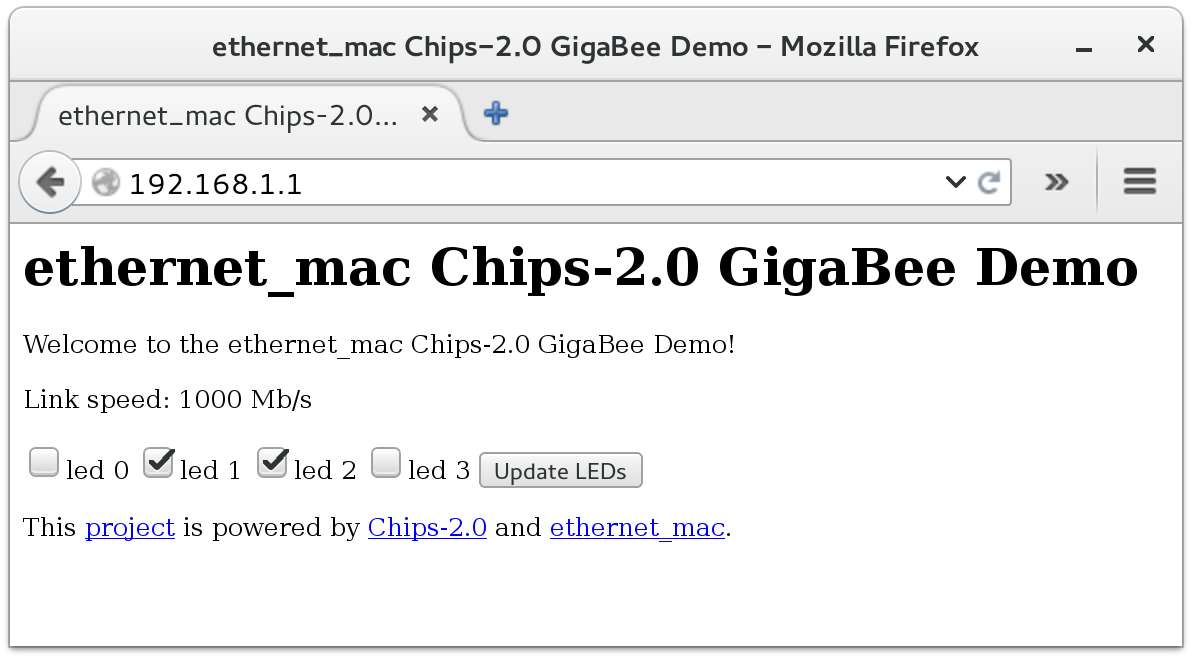
\includegraphics[width=0.8\textwidth]{Figures/chipsweb.png}
\caption{Index page of the modified Chips webserver demo project using the MAC sublayer presented in this thesis}
\label{fig:chipsweb}
\end{figure}

After downloading the design onto the FPGA, a standard web browser was pointed at the static IP address set in the C code. \fref{fig:chipsweb} shows a screenshot of the resulting web page. Pressing the ``Update LEDs" button changes the state of the light emitting diodes on the baseboard as expected. The test was successfully repeated at 10 and 100~Mb/s link speed.

\section{FPGA resource and code statistics}

On the test platform, the fully routed design including the loopback benchmark application consumed the resources we see in \tref{table:mac_res}. The amount of available units is different for most other members of the Spartan-6 family and is included only as an indicator for how much logic is left for actual user applications on the smallest GigaBee micromodule. Also, the number of used resource units will vary greatly when the MAC is ported to other FPGA families.

Although it was decisively not a goal of the present thesis, the utilization of FPGA resources is quite small as a consequence of the minimal feature set.

The complete core of the MAC sublayer (without any user application) was implemented in 2,275 lines of actual VHDL code not including blank lines and 531 additional lines of comments. The testbench additionally needs 869 lines of code and 149 lines of comments. In other words, comments make up approx.\ 18 percent of all lines and verification code accounts for about 28 percent of the lines of code.

\begin{table}
\caption{MAC sublayer resource usage (including minimal encompassing user design) on the Xilinx Spartan-6 family FPGA XC6SLX45-2FGG484}
\centering
\begin{tabu} to\linewidth {lrr}%X[2]X[r]X[2r]}
\rowfont[c]{\bfseries} Resource & Used & Total available \\ \hline
Slice registers & 603 & 54,576 \\
Slice LUTs & 882 & 27,288 \\
Occupied slices & 349 & 6,822  \\
RAMB16BWERs (block RAM) & 3 & 116 \\
BUFG/BUFGMUXs & 3 & 16 \\
DCMs & 1 & 8 \\
\end{tabu}
\label{table:mac_res}
\end{table}

\chapter{Conclusion}\label{ch:conclusion}
%Were the goals reached? -> Throughput (data rate), easy to understand
% Meinen Anteil herausstellen -> nicht in der Einleitung!

This thesis presented an Ethernet MAC sublayer design and corresponding implementation in VHDL that was devised primarily with simplicity in mind, both in external usage and in internal operation. Smaller applications that want to use Ethernet directly from the HDL code such as the transmission of measurement data in a network of ultra-wideband sensors will benefit from the simple FIFO interface offered while nevertheless being able to send and receive at almost full Gigabit Ethernet speed.

The MAC supports communicating with a physical layer integrated circuit via the standard media-independent interface at 10, 100, and 1000~Mb/s link speed and automatic detection of the current speed. Prior FPGA implementations of tri-mode Ethernet MAC sublayers were laden with nonessential features such as CSMA/CD for half-duplex connections, energy-efficient Ethernet support, or complex on-chip bus interfaces. While beneficial for e.g. using them in combination with embedded processors, an increasing amount of features is accompanied by increasing complexity and cost. In contrast, only essential Ethernet functionality was considered for the present thesis.

%Ethernet is a mature communication and networking technology with a sizable number of advantages for networks of ultra-wideband sensors and many other use cases when compared to competing solutions such as the universal serial bus (USB). Applications that want to use it can employ the help of a media access control sublayer that abstracts the details of getting packets from and to the network.

The design discussion demonstrated how ease of use and understanding were achieved in practice. We have seen that the tasks the Ethernet MAC has to perform were clearly separated into a concise structure of VHDL entities. The user interface is comprised of two FIFO buffers with well-known and simple interfaces for sending and receiving packets respectively. To avoid requiring the user to process invalid data, broken packets received from the network are dropped internally. All functionality is wrapped in a single  entity called \texttt{ethernet\_with\_fifos} that the user can instantiate into his or her design with little effort.
\clearpage
We then reviewed the implementation of MII I/O functionality on the Xilinx Spartan-6 family FPGA used in the primary target platform, the Trenz Electronic GigaBee micromodule. Architectures were presented for both transmission and reception that allow dynamic switching between MII and GMII and provide sufficient performance even at 1000~Mb/s link speed.

For the FIFO buffers facing the user, a generated standard implementation was chosen for the TX direction and a custom one for the RX direction because it was the best way to ensure a consistent, symmetrical interface. By synchronizing the read and write pointers per packet transaction, the complexity of using grey counters usually needed for asynchronous FIFOs was avoided.

A self-checking VHDL testbench confirmed that all basic functionality was implemented correctly. To 
ensure that no major speed limitations emerged as a consequence of keeping the design simple, a benchmark was performed which clearly proved that performance very close to the theoretical maximum is reached at all three supported link speeds. Finally, integrating the MAC sublayer into an existing web-server demo project with little effort has shown us that applications can make use of the core easily.

The resulting source code is published on the online collaboration platform GitHub~\cite{GithubMAC} under an open-source license. The preceding chapters specifically described the state found at~\cite{GithubMACCommit}, but further updates to the code might be made in the future. To the knowledge of the author, this is the first VHDL tri-mode Ethernet MAC implementation available without any license fee. One free Verilog alternative exists at OpenCores~\cite{MAC_opencores}, but its design goals are severely different.

While attention was paid to the secondary goal of making large parts of the IP core device-independent, the TX FIFO is not completely satisfactory in this regard. It relies on the proprietary LogiCORE generator that will only work with Xilinx FPGAs. Although this was a deliberate choice for the sake of simplicity, it becomes a significant limitation when porting the MAC to FPGAs of other vendors. Future work should provide a custom implementation similar to the RX FIFO directly in VHDL code as an alternative where using the Xilinx FIFO is unfeasible.

% heise: p. 347
Although all basic Ethernet functionality is included, some secondary features were left out. Half-duplex operation is highly unlikely to be encountered in modern networks, but flow control functionality is certainly desirable when operating at high data rates. The IEEE standard even recommends that every Gigabit Ethernet component supports flow control~\cite{heiseEthernet}. However, care must be taken to reach a fair compromise between the benefit of additional features and the complexity they introduce. While it should be possible to integrate flow control into the existing design with only minor modifications to the current entities by adding a component that handles the transmission and reception of the corresponding control frames, doing so is expected to compromise the clarity of the present MAC sublayer too much. In contrast, additional interfaces to the PHY such as the reduced gigabit media-independent interface (RGMII) should not pose a problem since they can be implemented by replacing the \texttt{mii\_gmii} and \texttt{mii\_gmii\_io} entities without adding additional components at all.

An aspect of media access control functionality that has received little attention in the present thesis is the addressing of nodes on the network. All packets received from the PHY are handed to the user, no matter whether they were ultimately destined for the device or not. He or she is then responsible for checking the destination address and acting accordingly. The amount of non-matching data received will be small because Ethernet switches generally forward packets only to the switch port corresponding to the destination address anyway. Nevertheless, dropping packets meant for other network nodes inside the MAC sublayer already should be considered to further improve user-friendliness. Similarly, outgoing packets need a valid source address that could be inserted automatically by the IP core.

When we take a look at the bigger picture, we observe that Ethernet is rarely used by itself without at least network and transport protocols such as IP and TCP. The ultra-wideband sensor networks which this Ethernet MAC was primarily developed for are no exception. Consequently, most users will have an additional demand for an FPGA core that realizes this functionality, so that only the actual application layer functionality is left for them to implement. Quite similar to the original problem statement that led to this thesis, simple and understandable hardware TCP/IP implementations for FPGAs are scarce. Future work should investigate which features of which higher-layer protocols are essential for basic applications and how they can be implemented in cooperation with the MAC sublayer presented in this thesis in a straightforward manner to offer a comprehensive solution for Ethernet communication.

% CRC32 nach 00 01 02 03 04 05 00 00 (z.B. 6 Byte mit 2 Byte Padding): 0xC3408C97
% -> komplementär: 0x5D5A2902
% -> umgedreht   : 0x40945ABA

% CRC32 nach 00 01 02 03 04 05 06 00 (z.B. 7 Byte mit 1 Byte Padding): 0xC3408C97
% -> komplementär: 0x3CBF7368
% -> umgedreht   : 0x16CEFD3C

% CRC32 nach 00 01 02 03 04 05 06 07 (z.B. 8 Byte mit 0 Byte Padding): 0x06E9AAEE
% -> komplementär: 0xF9165511
% -> umgedreht   : 0x88AA689F

%% ----------------------------------------------------------------
% Now begin the Appendices, including them as separate files

\addtocontents{toc}{\vspace{2em}} % Add a gap in the Contents, for aesthetics

\appendix % Cue to tell LaTeX that the following 'chapters' are Appendices

% Kürzere Codefragmente im Fließtext, längere im Anhang
% ganzer Code muss _nicht_ rein!

% Zitierstil: seq. Nummer in Klammern

%\input{Appendices/AppendixA}	% Appendix Title

\chapter{Timing Diagrams}\label{ch:framing_timing}

The following diagrams show the detailed timing when interacting with the \texttt{framing} entity from the user (FIFO) side. 4 bytes of data are transmitted or received respectively. The \texttt{mii\_gmii} side is identical for reception and only differs in the missing \texttt{tx\_busy} signal for transmission. The meaning of the signals is provided in \sref{ch:framing} and, more specifically, in \tref{table:framing_signals}.

\section{Transmission}

\begin{figure}[h]
%\large
\begin{tikztimingtable}[timing/font=\ttfamily]
	tx\_clock      & 13{C}                                          0.5C ;[dotted] 2H; 4{C} \\
	tx\_enable     & 1.5L 8H                                          4L ;[dotted] 2L; 4L \\
	tx\_data       & 1.5U 2D {$D_0$} 2D {$D_1$} 2D {$D_2$} 2D {$D_3$} 4U ;[dotted] 2U; 4U \\
	tx\_byte\_sent &    2L 8H                               3.5L         ;[dotted] 2L; 4L \\
	tx\_busy       & 3.5L       10H                                      ;[dotted] 2H; 1.5H 2.5L \\
\end{tikztimingtable}
\caption{Transmission of a frame when GMII is used}
\end{figure}

\begin{figure}[h]
%\large
\begin{tikztimingtable}[timing/font=\ttfamily]
	tx\_clock      & 19{C}                                          0.5C ;[dotted] 2H; 4{C} \\
	tx\_enable     & 1.5L 16H                                         2L ;[dotted] 2L; 4L \\
	tx\_data       & 1.5U 4D {$D_0$} 4D {$D_1$} 4D {$D_2$} 4D {$D_3$} 2U ;[dotted] 2U; 4U \\
	tx\_byte\_sent & 3.5L      4{2H2L}                                   ;[dotted] 2L; 4L \\
	tx\_busy       & 3.5L      16H                                       ;[dotted] 2H; 1.5H 2.5L \\
\end{tikztimingtable}
\caption{Transmission of a frame when MII is used}
\end{figure}

\clearpage
\section{Reception}

\begin{figure}[h]
%\large
\begin{tikztimingtable}[timing/font=\ttfamily]
	rx\_clock          & 13{C}                                               \\
	rx\_frame          & 1.5L 8H                                          4L \\
	rx\_data           & 1.5U 2D {$D_0$} 2D {$D_1$} 2D {$D_2$} 2D {$D_3$} 4U \\
	rx\_byte\_received & 1.5L 8H                                          4L \\
\end{tikztimingtable}
\caption{Reception of a frame when GMII is used}
\end{figure}

\begin{figure}[h]
%\large
\begin{tikztimingtable}[timing/font=\ttfamily]
	rx\_clock          & 20{C}                                                        \\
	rx\_frame          & 1.5L 16H                                                  3L \\
	rx\_data           & 3.5U 2D {$D_0$} 2U 2D {$D_1$} 2U 2D {$D_2$} 2U 2D {$D_3$} 3U \\
	rx\_byte\_received & 3.5L      4{2H2L}                                         1L \\
\end{tikztimingtable}
\caption{Reception of a frame when MII is used}
\end{figure}

\chapter{Coding Style}\label{ch:coding_style}

A consistent coding style makes the code considerably easier to grasp both locally and in its entirety. To that effect, the following principles have been applied consistently throughout the source code:
\begin{itemize}
\item Expressive names for signals, variables, constants etc.
\item Prefixing type names with \texttt{t\_} and suffixing all entity port names with their respective direction (\texttt{\_i} for input, \texttt{\_o} for output, or \texttt{\_io} for both)
\item Usage of the standard IEEE package \texttt{ieee.numeric\_std} instead of vendor-specific ones for mathematical functions
\item Putting types, constants, and functions common to multiple entities into shared packages instead of repeating them
\item Distinct usage of signals for storage and variables for intermediate values
\item Usage of generics and type attributes for flexibility
\item Simple one-process unified coding style for finite state machines by default, usage of two processes where they provide an easier representation of the functionality
\item Comments where they add meaningful information beyond the obvious operation performed by the code
\item Indentation with tabulator characters
\end{itemize}

%\input{Appendices/AppendixB} % Appendix Title

%\input{Appendices/AppendixC} % Appendix Title

\addtocontents{toc}{\vspace{2em}}  % Add a gap in the Contents, for aesthetics
\backmatter

%% ----------------------------------------------------------------
\label{Bibliography}
\lhead{\emph{Bibliography}}  % Change the left side page header to "Bibliography"
%\bibliographystyle{unsrtnat}  % Use the "unsrtnat" BibTeX style for formatting the Bibliography
%\bibliography{Bibliography}  % The references (bibliography) information are stored in the file named "Bibliography.bib"
\printbibliography

\end{document}  % The End
%% ----------------------------------------------------------------
